\documentclass[11pt,a4paper]{article}
\usepackage[T1]{fontenc}
\usepackage{lmodern,microtype}
\usepackage[margin=28mm]{geometry}
\usepackage{amsmath,amssymb,amsthm,mathtools}
\usepackage{booktabs,longtable,array,enumitem}
\usepackage[numbers,sort&compress]{natbib}
\usepackage[hyphens]{url}
\usepackage{xurl}
\usepackage[hidelinks]{hyperref}
\usepackage{bookmark}
\usepackage{tikz}
\usetikzlibrary{arrows.meta,positioning}
\hypersetup{pdftitle={A fixed-target approach to the sharp iid Berry--Esseen inequality},
 pdfauthor={Bartosz Kołodziejek and Kacper Rodziewicz}}
\setlength{\emergencystretch}{2em}
\linespread{1.06}
\setlength{\parskip}{2pt plus 1pt minus .5pt}
\setcounter{tocdepth}{1}
\makeatletter
\renewcommand\paragraph{\@startsection{paragraph}{4}{\z@}%
  {2.5ex \@plus1ex \@minus.2ex}{0.8ex \@plus.2ex}%
  {\normalfont\normalsize\bfseries}}
\makeatother
\newcolumntype{P}[1]{>{\raggedright\arraybackslash}p{#1}}
\newtheorem{theorem}{Theorem}[section]
\newtheorem{lemma}[theorem]{Lemma}
\newtheorem{proposition}[theorem]{Proposition}
\newtheorem{corollary}[theorem]{Corollary}
\theoremstyle{definition}
\newtheorem{definition}[theorem]{Definition}
\newtheorem{assumption}[theorem]{Assumption}
\newtheorem{condition}[theorem]{Certificate condition}
\theoremstyle{remark}
\newtheorem{remark}[theorem]{Remark}
\newcommand{\E}{\mathbb E}
\newcommand{\Pp}{\mathbb P}
\newcommand{\R}{\mathbb R}
\newcommand{\N}{\mathbb N}
\newcommand{\CE}{C_{\mathrm E}}
\newcommand{\supp}{\operatorname{supp}}
\newcommand{\Var}{\operatorname{Var}}
\newcommand{\pos}[1]{(#1)_+}
\newcommand{\ind}{\mathbf 1}
\newcommand{\iid}{\mathrm{iid}}
\title{A fixed-target approach to the sharp iid\\
Berry--Esseen inequality\thanks{This paper was written with substantial
assistance from AI systems; see the end of Section~\ref{ms:discussion}.}}
\author{Bartosz Ko{\l}odziejek \and Kacper Rodziewicz}
\date{29 October 2026}
\begin{document}
\maketitle
\begin{abstract}
We study the conjectured sharp iid Berry--Esseen constant by maximizing
excess over its fixed target. Attainment and contact give a common
moment-defect budget; a specified Fourier certificate supplies coarse
entry. For $n\ge700$, direct geometry and two contact rays acquire one
support strip. A single-count fourth-moment bound handles small noise,
and a five-count identity handles the rest. Both comparisons preserve
the actual marginal, threshold atoms and complete tails. The resulting
global implication remains conditional on the stated entry predicates
and a genuine finite base through $699$, which is not proved here.
\end{abstract}
\section{The problem, results, and proof strategy}\label{ms:introduction}
\subsection{The problem and the candidate constant}
Let $\mathcal P$ be the laws on $\R$ with mean zero, variance one and
finite third absolute moment $\rho(P)=\E|X|^3$. For independent copies
$X_1,\ldots,X_n$ of $P$, put $S_n=\sum_iX_i$ and
\[
 \Delta_n(P)=\sup_{H\in\R}|\Pp_P(S_n\le H)-\Phi(H/\sqrt n)|,
 \qquad C_n=\sup_{P\in\mathcal P}\frac{\sqrt n\,\Delta_n(P)}{\rho(P)}.
\]
Here $\Phi$ and $\phi$ are the standard normal distribution function
and density. The sharp-constant conjecture is
\begin{equation}\label{ms:conjecture}
 \sup_{n\ge1}C_n=\CE,
 \qquad \CE=\frac{3+\sqrt{10}}{6\sqrt{2\pi}}=0.409732\ldots.
\end{equation}
Throughout, $H$ is a threshold for the unnormalized sum $S_n$, and
a terminating decimal in an inequality denotes the corresponding exact
rational number. Affine standardization gives the equivalent result
for any mean and positive variance, with third absolute central moment
divided by the cube of the standard deviation.

Berry and Esseen established the classical order $n^{-1/2}$
\cite{Berry1941,Esseen1942,Esseen1945}. Esseen's lower bound
\cite{Esseen1956} explains the proposed constant. If
$p_*=(4-\sqrt{10})/2$, $q_*=1-p_*$ and
$X=(B-p_*)/\sqrt{p_*q_*}$ for $B\sim\operatorname{Bernoulli}(p_*)$,
the fixed-law lattice limit gives
\begin{equation}\label{ms:bernoulli-limit}
 \lim_{n\to\infty}\frac{\sqrt n\Delta_n(P)}{\rho(P)}
 =\frac{3+q_*-p_*}{6\sqrt{2\pi}(p_*^2+q_*^2)}=\CE.
\end{equation}
Indeed $p_*^2+q_*^2=10-3\sqrt{10}$ and
$(3+q_*-p_*)/(p_*^2+q_*^2)=3+\sqrt{10}$.
Every constant below $\CE$ therefore fails for a sufficiently large sum
of this one law. The upper conjecture is associated with Zolotarev
\cite{Zolotarev1966,Zolotarev1967}; Schulz proves the strict finite-index
bound for every nondegenerate Bernoulli law \cite{Schulz2016}.


\subsection{Results and their hypotheses}\label{ms:scope}
The results have three distinct roles. We state their interfaces here;
the cited theorems give their complete hypotheses and proofs.
\begin{center}\small
\begin{tabular}{@{}P{.25\linewidth}P{.68\linewidth}@{}}
\toprule
Result & Conclusion and required inputs \\
\midrule
Local comparison, Theorem~\ref{short:count:local} &
For $n\ge700$, every law in its specified conditional-support region,
with $p\in[3/8,93/200]$, $0<\lambda\le7/20$ and $|H|\le46/25$,
has excess below $-\lambda/100$. The zero-noise excess is strictly
negative. This statement uses only its explicit law hypotheses. \\
Localization, Theorem~\ref{v9:entry:theorem} &
A maximizer with nonnegative excess at $n\ge42$ satisfies
$nD\le32.20665378$ and $|H|\le1.83605680$, under
$C_{n-1}\le\CE$, the structural inequality and the two stated
finite-verification conditions. \\
Global implication, Theorem~\ref{short:global} &
With the retained structural, binomial and finite-verification inputs,
a base $C_j\le\CE$ for every $j\le699$ implies $C_n<\CE$ for
$n\ge700$ and $\sup_n C_n=\CE$. The finite base remains open here. \\
\bottomrule
\end{tabular}
\end{center}
The structural input is displayed in \eqref{v9:entry:structural}; the
finite-binomial input is \eqref{short:count:binomial}.
Conditions~\ref{v9:entry:two-pass-condition} and
\ref{v9:entry:signed-condition} specify the finite localization
checks. Their exact replay is recorded in Appendix~\ref{revision:reproducibility}.
The analytical reduction, the whole-domain coverage, and the
correspondence of the checking code with those inequalities are the
components of this computational proof. We retain these premises
explicitly in the theorem statements.

\subsection{Why the defect controls a maximizer}
At a fixed $n$, maximize the difference between the two sides of the
candidate inequality:
\begin{equation}\label{v9:intro:excess}
 a(P,H)=\sqrt n\{\Pp_P(S_n\le H)-\Phi(H/\sqrt n)\}-\CE\rho(P).
\end{equation}
Proposition~\ref{v9:core:attainment} proves attainment. Its first-order
condition bounds $y\mapsto\Pp(S_{n-1}\le H-y)$ by an explicit
piecewise cubic function that agrees with it on the closed support.
This contact condition allows us to use the geometry of that support.

Let $\tau(t)=\E[X\ind_{\{X\ge t\}}]$ be the zero-bias density and
$J=\sum_g\tau_g|g|^2$, where $g$ runs over bounded support gaps and
$\tau_g$ is the constant value of $\tau$ there. A lattice law of span
$h$ has $J\ge h$; if every successive gap has length $h$, then $J=h$.
Thus $J$ measures gap size with zero-bias weights. The inequality
\[
 \gamma+3J\le(3+\sqrt{10})\rho,\qquad \gamma=\E X^3,
\]
proved in Lemma~\ref{ms:physical-defect}, extends the moment--span
bound from lattice laws to arbitrary standardized laws. Its slack
\[
 D=(3+\sqrt{10})\rho-\gamma-3J
\]
is nonnegative and vanishes exactly at the positive-skew Bernoulli
law in \eqref{ms:bernoulli-limit}. The lattice consequence and its
reflection are proved in Corollary~\ref{opus:lattice-gap}.

Integrating the contact relation against $\tau$ in two ways gives the
conservation identity of Theorem~\ref{revision:contact-conservation}.
Since $\CE=(3+\sqrt{10})\phi(0)/6$, its two leading moment terms
combine into a multiple of $D$. Solving for the excess gives
\[
 a=\frac{\mathcal R_c-n\CE\rho(1-e)
             -n\phi(0)eD/6-n^{3/2}L}{n+H^2},
 \qquad e=\exp(-H^2/(2n)).
\]
Here $L\ge0$ is a weighted contribution from the law of $H-S_{n-1}$
inside the support gaps, and $\mathcal R_c$ is an explicitly defined
remainder. The three subtracted terms are nonnegative. A nonnegative
excess therefore requires $n\phi(0)eD/6\le\mathcal R_c$.
Once localization bounds both $\mathcal R_c$ and $|H|$, this bounds
$nD$. The uniform bounds come from Theorem~\ref{v9:entry:theorem},
not from a fixed-law asymptotic expansion.

The predecessor hypothesis supplies an upper bound for
$\Pp(S_{n-1}\le H-t)$ in the contact condition, which excludes remote
support points; see \eqref{v9:entry:contact}. This support argument is
used both in coarse localization and in the final two-ray estimate.
With $nD\le32.20665378$, the geometry at $n\ge700$ gives
$3/8<p<93/200$, inward support displacement below $1/250$ and
$\lambda<7/20$. Count conditioning then compares the law with a
binomial sum. One threshold count controls noise up to $1/100$;
five neighboring counts control the remaining interval. Both
comparisons keep all probabilities entering from other counts.

\begin{figure}[ht]
\centering
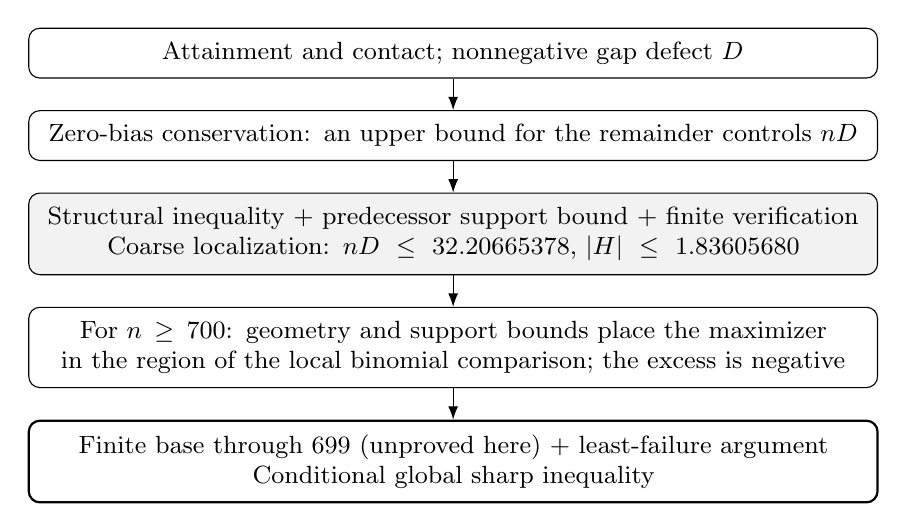
\begin{tikzpicture}[node distance=4mm,>=Latex,
 box/.style={draw,rounded corners,align=center,text width=.86\linewidth,
 inner sep=5pt,font=\small}]
\node[box] (contact) {Attainment and contact; nonnegative gap defect $D$};
\node[box,below=of contact] (identity) {Zero-bias conservation: an upper bound for the remainder controls $nD$};
\node[box,fill=gray!10,below=of identity] (entry) {Structural inequality + predecessor support bound + finite verification\\
Coarse localization: $nD\le32.20665378$, $|H|\le1.83605680$};
\node[box,below=of entry] (local) {For $n\ge700$: geometry and support bounds place the maximizer\\
in the region of the local binomial comparison; the excess is negative};
\node[box,line width=.8pt,below=of local] (global) {Finite base through $699$ (unproved here) + least-failure argument\\
Conditional global sharp inequality};
\draw[->] (contact)--(identity);
\draw[->] (identity)--(entry);
\draw[->] (entry)--(local);
\draw[->] (local)--(global);
\end{tikzpicture}
\caption{The proof's dependencies. The shaded step uses the specified
finite verification; the final step also requires the unproved finite base.
The local comparison is a theorem for its explicit law region, independently
of the preceding localization.}
\label{opus:proof-flow}
\end{figure}

\FloatBarrier
\subsection{The computer-assisted localization}
Analysis restricts a possible maximizer to a bounded moment region.
It also bounds the remainder by functions of moment and support
parameters. The computation encloses these functions on finitely many
closed boxes. Each box is either excluded by a necessary inequality,
or assigned bounds valid throughout that box. The boxes cover their
parent regions, including shared boundaries, so every possible
maximizer retains a valid bound.

The certificate is a compact record of this process. It stores
checkpoints for $24$ third-moment cells over four signed-moment passes,
including support radii, bounds and descendant counts; the individual
$11264$ nominal boxes are reconstructed. Two preliminary coarse passes
are reconstructed as well. The exporter chooses a successful sequence
of passes and rounds its reported bounds outward. The acceptor
recomputes the prescribed subdivisions and verifies their inequalities
and output bounds.

All numerical acceptance uses integers and exact rational numbers,
with directed rational enclosures for roots, exponentials and Gaussian
constants. The exploratory program and the checker share the routine
\texttt{signed\_core.stage}; acceptance is an exact replay of that
calculation. Independent checking requires auditing these routines
against the mathematical rules or implementing those rules separately.
Appendix~\ref{revision:reproducibility} gives a code-reading guide,
reproduction commands and the recorded execution environment.

Subdivision and rigorous enclosure have established precedents in
computer-assisted proofs \cite{SolovyevHales2013}. Numerical optimization
also appears in Berry--Esseen estimates \cite[Section~2]{Shevtsova2011}.
The custom JSON format organizes this calculation; the rigor comes from
the valid enclosures, coverage and correct implementation of the rules.

\subsection{Related work}
Fourier and structural moment inequalities progressively improved the
universal upper bound \cite{vanBeek1972,Prawitz1972,Tyurin2010,
Shevtsova2011,Shevtsova2013}. We use Shevtsova's structural inequality
explicitly in localization. Recent manuscripts report smaller upper
constants \cite{xiao2026berryesseen,lin2026berryesseen}, and He and Cheng
report eventual sharpness beyond a uniform, very large threshold
\cite{hecheng2026eventually}. Work on independent arrays and extremizers
addresses the related non-iid problem \cite{BellIndependent2026,
BellExtremizers2026}. These recent reported results are not used in
our proof. An earlier AI-assisted working draft is on Hexagon
\cite{rodziewiczkolodziejek2026momentdefects}.

\section{Fixed-target extremizers and contact}
\label{v9:core:section}

We optimize the excess above a fixed candidate constant. This gives a
variational problem whose coefficient is known before any acquisition
step. The positive excess is retained through the contact calculation
and the conserved identity; it becomes a nonnegative term in the final
resource. No upper bound for the maximizing normalized score is needed.
Throughout, sums have
independent identically distributed summands with mean zero, variance one
and finite third absolute moment $\rho$. Fix $n\ge2$, $c>0$, and a real
raw sum threshold $H$. Set
\begin{gather*}
 z=H/\sqrt n,\quad F=\Pp(S_n\le H),\quad
 a=\sqrt n\{F-\Phi(z)\}-c\rho,\\
 \varphi=\phi(z),\quad\beta=\E[X|X|],\quad\gamma=\E X^3.
\end{gather*}
In particular $a$ is not divided by $\rho$.

\subsection{Attainment, contamination and the entire closed support}

\begin{proposition}\label{v9:core:attainment}
For each fixed $n$ and $c>0$, the supremum of $a$ over these laws and
thresholds is attained, and the closed-CDF discrepancy at every attaining
pair is positive.
At every maximizing pair,
\begin{align}
 I(y)={}&n^{3/2}\{h(y)-F\}+ny\varphi
       +\tfrac12H\varphi(y^2-1)\notag\\
 &+\tfrac32c\rho(y^2-1)-c\{|y|^3-\rho-3y\beta\}\le0,
 \qquad h(y)=\Pp(S_{n-1}\le H-y),\label{v9:core:contact}
\end{align}
with equality on the whole closed support. That support is compact.
Neither statement assumes $a\ge0$ or $H\ge0$.
\end{proposition}
\begin{proof}
Write $A$ for the supremum. Since $\rho\ge1$ and the discrepancy is
at most one, $A\le\sqrt n-c$. Symmetric Bernoulli evaluated at $H=n$
gives $A\ge\sqrt n(1-\Phi(\sqrt n))-c>-c$.
For a maximizing sequence, $a_j\to A$ and
$c\rho_j\le\sqrt n-a_j$ give a common third-moment ceiling.
The discrepancies satisfy $\sqrt n(F_j-\Phi(H_j/\sqrt n))
=a_j+c\rho_j\ge a_j+c>\eta$ eventually for some $\eta>0$.
Chebyshev bounds the negative threshold tail by $n/H_j^2$;
the positive discrepancy is at most the normal tail, also at most
$n/H_j^2$. Thus $H_j$ is bounded.

Tightness gives a subsequence $P_j\Rightarrow P$, $H_j\to H$ and
$\rho_j\to b$. The common third-moment ceiling $M$ gives tail
bounds $\int_{|x|>K}x^2dP_j\le M/K$ and
$\int_{|x|>K}|x|dP_j\le M/K^2$. Bounded continuous truncations
therefore preserve mean and variance. Lower semicontinuity gives
$1\le\rho(P)\le b$. For fixed $n$, the sum laws converge weakly.
Applying the closed-set inequality first at $H+t$ and then letting
$t\downarrow0$ gives
$\limsup F_j(H_j)\le F_P(H)$, including an atom at $H$.
Consequently
\[
 a(P,H)\ge A+c\{b-\rho(P)\}\ge A.
\]
Maximality forces equality and $\rho(P)=b$. Convergence of third
moments is a conclusion here; it was not inferred from bounded third
moments. The discrepancy remains positive since $A+c\rho\ge A+c>0$.

The contact inequality is a first-variation condition. To obtain it,
contaminate the raw marginal by
$(1-\epsilon)P+\epsilon\delta_y$. Its mean is $\epsilon y$,
variance $v_\epsilon=1+\epsilon(y^2-1)-\epsilon^2y^2$, and centered
third absolute moment has derivative $|y|^3-\rho-3y\beta$ at zero.
The last assertion follows by dominated differentiation of
$|x-\epsilon y|^3$, with bound $3|y|(|x|+|y|)^2$.
Evaluate the standardized law at the standardized image of the fixed
raw event $S_n\le H$. The raw event probability is a polynomial in
$\epsilon$, with derivative $n(h(y)-F)$ even at an atom collision.
The normal argument is
$(H-n\epsilon y)/\sqrt{nv_\epsilon}$, whose derivative is
$-\sqrt n y-H(y^2-1)/(2\sqrt n)$.
The one-sided derivative of the excess is exactly \eqref{v9:core:contact};
maximality makes it nonpositive.

Its integral against $P$ is zero. All terms are integrable.
The closed-event map $h$ is upper semicontinuous; at an atom it takes
the larger one-sided value. Thus $I$ is upper semicontinuous. Strict
negativity at a closed-support point would hold with a uniform negative
margin on a neighborhood of positive $P$-mass, contradicting its zero
integral. Finally $I(y)\le-c|y|^3+C_2y^2+C_1|y|+C_0$ for constants
depending on this pair. It is strictly negative on both sufficiently
distant rays, proving compact support. No higher moments were used
before this step.
\end{proof}

\subsection{Reflection, equality, and the first unresolved index}
\label{v9:core:reflection}
The sign of the attained maximum detects failure of a strict row bound,
including equality. If $C_n$ denotes the supremum of the normalized
absolute discrepancy, reflection gives, including an atom at $H$,
\[
 \Pp(-S_n\le-H)-\Phi(-z)
 =\Phi(z)-\Pp(S_n<H)\ge\Phi(z)-F.
\]
Thus each negative closed-CDF error is bounded by a positive closed-CDF
error of the reflected law; equality at an atom is not assumed.
Consequently $C_n$ is also the supremum of positive
closed scores $r$. Since $a=\rho(r-c)$, $C_n<c$ gives
$A\le C_n-c<0$, and $C_n>c$ gives $A>0$. If $C_n=c$, choose
$r_j\uparrow c$ with $r_j\ge c/2$. Then
$\rho_j\le2\sqrt n/c$, so $\rho_j(r_j-c)\to0$ and $A=0$.
Hence $C_n\ge c$ supplies an attained pair with $a\ge0$.

\begin{corollary}[First failure of a strict bound]\label{v9:core:first-failure}
Assume a genuine finite base $C_j\le c$ for $1\le j<N$. If a strict
bound $C_n<c$ fails at any index $n\ge N$, there is a least such index,
an attained fixed-target pair with $a\ge0$, and true predecessor bounds
$C_j\le c$ for every $j<n$. The bounds are strict for $N\le j<n$.
\end{corollary}
\begin{proof}
The nonempty set of failing indices at least $N$ has a least member.
The preceding equivalence supplies its maximizing pair. Indices below
$N$ use the finite base; the other earlier indices use minimality.
\end{proof}
Thus an argument excluding every such pair for $n\ge N$ would give
strict bounds above the finite base, including exclusion of equality.
The subsequent entry argument uses only $C_{n-1}\le c$; it does not
use an upper bound for the actual score $c+a/\rho$. The finite base
and the eventual exclusion remain separate obligations.

Equivalently, $\Delta=Q-h\ge0$ everywhere and $\Delta=0$ on the closed
support, where
\begin{equation}\label{v9:core:Q}
 Q(y)=F+\frac{H\varphi+c\rho}{2n^{3/2}}
 -\frac{n\varphi+3c\beta}{n^{3/2}}y
 -\frac{H\varphi+3c\rho}{2n^{3/2}}y^2
 +\frac c{n^{3/2}}|y|^3.
\end{equation}

\section{The two-point skeleton and its moment defect}
\label{ms:geometry-counts}

Every centered law can be separated into its positive and nonpositive
parts. Replacing each part by its conditional mean gives a two-point law;
the remaining conditional fluctuations measure its departure from that
law. We first make this decomposition exact, then identify a moment
defect that vanishes at Esseen's extremal distribution.

\subsection{The sign split and its units}

Fix $P\in\mathcal P$ and put
\[
 p=\Pp(X>0),\quad q=1-p,\quad v=pq,\quad
 m=\E X_+=\E X_->0,\quad B_0=\mathbf1_{\{X>0\}}.
\]
Both $p,q$ are positive; a possible atom at zero is assigned to the
nonpositive class. Define $V=\E[X\mid B_0]$ and $W=X-V$, so that
\[
 V=-m/q\quad(B_0=0),\qquad V=m/p\quad(B_0=1),\qquad
 \theta=\E W^2=1-m^2/v<1.
\]
Write $\theta_-=\E[W^2;B_0=0]$ and $\theta_+=\E[W^2;B_0=1]$.
The distance between the two conditional means is
\[
 \ell=m/v=\sqrt{(1-\theta)/v}>0.
\]
Set $U=W/\ell$, $Y=B_0+U$, and $s=\E U^2$. Then
\begin{subequations}\label{ms:bernoulli-coordinates}
\begin{align}
 X&=\ell(Y-p)=\frac{B_0+U-p}{\sqrt{pq+s}},\qquad
 \E[U\mid B_0]=0,\label{revision:canonical-decomposition}\\
 1&=pq\ell^2+\theta,\qquad s=\theta/\ell^2,\qquad
 v+s=\ell^{-2}.\label{short:acq:normalization}
\end{align}
\end{subequations}
Let $U_0,U_1$ have the two conditional laws, and put
\[
 w_i=\E U_i^2,\quad \mu_i=\E U_i^3,\quad
 s=qw_0+pw_1=\frac{v\theta}{1-\theta},\quad
 \lambda=ns.
\]
The moments $\mu_i$ are finite because $\rho<\infty$. Higher moments
will be used only after bounded support is known: for extremizers this
follows from Proposition~\ref{v9:core:attainment}, and for the local
comparison it is an explicit hypothesis.

If $s=0$, both nonnegative conditional variances vanish, so $U_0=U_1=0$
almost surely. This is exactly the standardized Bernoulli law. If $s>0$,
the parameter $\alpha=pw_1/s$ lies in $[0,1]$ and gives
$w_0=s(1-\alpha)/q$, $w_1=s\alpha/p$.

The signs of $X$ are still those defining the two classes, so expansion
of the actual conditional moments gives
\begin{align}
 \rho/\ell^3&=v(1-2v)+3v(w_0+w_1)-q\mu_0+p\mu_1,\notag\\
 \gamma/\ell^3&=v(q-p)+3v(w_1-w_0)+q\mu_0+p\mu_1,\notag\\
 \beta/\ell^2&=v(q-p)+pw_1-qw_0.
\label{ms:conditional-moments}
\end{align}
For example, on the nonpositive class $|X|^3=\ell^3(p-U_0)^3$;
on the positive class it is $\ell^3(q+U_1)^3$. Conditional centering removes
the linear terms and gives the first identity; the other two follow in
the same way. The three identities share the same pair $(\mu_0,\mu_1)$.

\subsection{A nonnegative moment defect}

The constant $3+\sqrt{10}$ has a simple geometric explanation. The
signed third moment and the first absolute moment satisfy a circle
inequality; the lengths of the support gaps are controlled by the same
first absolute moment. Neither fact requires bounded support.

Define
\[
 \tau(t)=\E[X\mathbf1_{\{X\ge t\}}],\qquad \sigma=\sqrt{10}.
\]
For $t<0$, centering gives $\tau(t)=-\E[X\mathbf1_{\{X<t\}}]\ge0$;
for $t\ge0$ nonnegativity is immediate. Signwise Tonelli integration gives
\begin{equation}
 \int_\R\tau(t)\,dt=1,
 \qquad 2\int_\R|t|\tau(t)\,dt=\rho.
\label{ms:tau-moments}
\end{equation}
On each bounded complementary interval $(a,b)$ of the closed support,
$\tau$ is constant in the interior, with value $\tau_{a,b}$. Put
\begin{equation}
 J=\sum_{(a,b)}\tau_{a,b}(b-a)^2,
 \qquad D=(3+\sigma)\rho-\gamma-3J.
\label{ms:physical-defect-definition}
\end{equation}
There are at most countably many gaps; the next proof shows that the
nonnegative sum is finite. Endpoint atoms do not affect its integrals.

\begin{lemma}[A moment circle and the gap inequality]
\label{ms:physical-defect}
\label{ms:fourier:afcore:lem:physical-defect}
For every $P\in\mathcal P$,
\begin{equation}
 \gamma^2+(2m)^2\le\rho^2,\qquad J\le\rho+2m,
 \qquad \gamma+tJ\le\bigl(t+\sqrt{1+t^2}\bigr)\rho\quad(t>0).
 \label{ms:gap-family}
\end{equation}
The last constant is sharp. Equality holds exactly at the standardized
Bernoulli law with positive mass $p_t=(1+t-\sqrt{1+t^2})/2$.
In particular, $D\ge0$. If zero belongs to the support, then
$D\ge(\sigma-1)\rho$; hence $D<(\sigma-1)\rho$ implies a central
support gap $(-A_-,A_+)$ with $A_-,A_+>0$.
\end{lemma}
\begin{proof}
Write $a_\pm=\E X_\pm^2$ and $b_\pm=\E X_\pm^3$, so
$a_++a_-=1$, $b_++b_-=\rho$ and $b_+-b_-=\gamma$.
Cauchy--Schwarz on each sign class gives
$a_\pm^2\le mb_\pm$. It also gives
$m^2\le pa_+$ and $m^2\le qa_-$, where an atom at zero is included
in $q$. Thus
$m^2(1/a_++1/a_-)\le1$, or $m^2\le a_+a_-$.
Consequently $b_+b_-\ge(a_+a_-)^2/m^2\ge m^2$, proving the
circle inequality since $\rho^2-\gamma^2=4b_+b_-$.

Every gap on one side of zero satisfies
$(b-a)^2\le2\int_a^b|x|\,dx$.
If a central gap $(-A_-,A_+)$ exists, its weight is $m$ and its excess
over this integral is $2mA_-A_+$. Moreover
$0\le\E[(X+A_-)(X-A_+)]=1-A_-A_+$.
Summing the gap bounds by Tonelli proves $J\le\rho+2m$.
If zero is in the support there is no central gap, so $J\le\rho$.
Finally Cauchy--Schwarz in $\mathbb R^2$ gives
$\gamma+2tm\le\sqrt{1+t^2}\rho$, proving the family and the
assertions about $D$.

Equality in the circle forces equality in the two signwise Cauchy
bounds: the positive and negative parts are each concentrated at one
nonzero value. Equality in $m^2\le a_+a_-$ excludes mass at zero.
For such a law, with positive mass $p$ and $q=1-p$, one has
$J=\rho+2m$. Equality in the last Cauchy bound requires
$\gamma=2m/t$, equivalently $t(1-2p)=2p(1-p)$.
Its unique solution in $(0,1)$ is the stated $p_t$.
\end{proof}

\begin{corollary}[The zero-defect law]\label{ms:zero-defect}
For $P\in\mathcal P$, $D=0$ if and only if
\[
 X=(B_0-p_*)/\sqrt{p_*q_*},\qquad
 p_*=(4-\sqrt{10})/2,\quad q_*=1-p_*,
 \quad B_0\sim\operatorname{Bernoulli}(p_*).
\]
\end{corollary}
\begin{proof}
Apply the equality case of Lemma~\ref{ms:physical-defect} with $t=3$.
\end{proof}

\begin{corollary}[The lattice consequence]\label{opus:lattice-gap}
Let $P\in\mathcal P$ be a lattice law with maximal span $h>0$. Then
\[
 J\ge h,\qquad |\gamma|+3h\le(3+\sqrt{10})\rho.
\]
Equality in the second inequality holds exactly for the law of
Corollary~\ref{ms:zero-defect} and its reflection. If successive support
points are all separated by $h$, then $J=h$.
\end{corollary}
\begin{proof}
The support is a closed subset of a translate of $h\mathbb Z$, so its
points have Lebesgue measure zero and every bounded gap has length
$k_gh$ for an integer $k_g\ge1$. The density $\tau$ vanishes outside
the convex hull of the support. Hence, by nonnegative integration,
\[
 \sum_g\tau_gk_gh=\int_\R\tau(t)\,dt=1,
 \qquad J=\sum_g\tau_gk_g^2h^2\ge h.
\]
These identities also hold for unbounded support: the gaps are
countable and their contributions increase to the full integral.
If all $k_g=1$, the inequality is an equality. Under reflection the
zero-bias density becomes $\tau(-t)$ almost everywhere. Thus reflection
preserves $\rho$, $J$ and $h$, and changes the sign of $\gamma$. Apply
Lemma~\ref{ms:physical-defect} to the orientation with nonnegative
third moment. Equality forces $D=0$, and the equality law has
$J=h$, so Corollary~\ref{ms:zero-defect} proves both directions.
\end{proof}
For a lattice law, $J$ is therefore a weighted average of support-gap
lengths, with weights $\tau_g|g|$ summing to one. The same functional
is defined for arbitrary support, which is why it can replace the
lattice span in the defect inequality.

In particular the defect separates two losses:
\[
 D=\underbrace{\sigma\rho-\gamma-6m}_{\text{moment loss}}
       +3\underbrace{(\rho+2m-J)}_{\text{gap loss}},
\]
each nonnegative. The point $(\gamma/\rho,2m/\rho)$ lies in the upper
unit disk. The line $x+3y=\sqrt{10}$ supports that disk at
$(1/\sqrt{10},3/\sqrt{10})$, explaining the coefficient in the moment
loss. For a standardized Bernoulli law with positive mass $p$, direct
calculation gives
\begin{align}
 J&=\frac1{\sqrt{pq}},&
 \rho_B(p)&=\frac{1-2pq}{\sqrt{pq}},\notag\\
 \gamma_B(p)&=\frac{q-p}{\sqrt{pq}},&
 D_B(p)&=\frac{(6+2\sigma)(p-p_*)^2}{\sqrt{pq}}.
 \label{ms:bernoulli-defect}
\end{align}
Indeed its zero-bias density is $\sqrt{pq}$ on the interval between its
two support points. The probability displacement therefore has a
quadratic cost. The equality proof above is what rules out other laws
with zero defect.

For quantitative estimates we need more information than their signs.
Suppose a central gap $(-A_-,A_+)$ has been established,
and write
\[
 T_+=\E X_+^3-mA_+^2,\quad T_-=\E X_-^3-mA_-^2,\qquad
 R_+=\E X_+^2-mA_+,\quad R_-=\E X_-^2-mA_-.
\]
These four quantities are nonnegative. For the outer gaps put
$J_o=J-m(A_-+A_+)^2$. A positive outer gap satisfies
$(b-a)^2\le2\int_a^b(t-A_+)\,dt$, so Tonelli gives
\[
 J_o^+\le2\int_{A_+}^\infty(t-A_+)\tau(t)\,dt
       =\E[X_+(X_+-A_+)^2]=T_+-2A_+R_+\le T_+.
\]
Similarly $J_o^-\le T_--2A_-R_-\le T_-$.
Expanding $D$, using $\sqrt{\sigma+1}\sqrt{\sigma-1}=3$, gives
\begin{align}
 D={}&m\{\sqrt{\sigma+1}A_--\sqrt{\sigma-1}A_+\}^2
       +(\sigma-1)T_++(\sigma+1)T_-\notag\\
    &+3(T_++T_--J_o).\label{ms:defect-decomposition}
\end{align}
Every term is nonnegative. Cauchy--Schwarz also gives
$1/(2\rho)\le m\le1/2$: indeed $1\le\rho\E|X|=2m\rho$ and
$\E|X|\le1$. Since $\sigma-1>2$, the decomposition yields
$T_++T_-\le D/2$. If $D<2$, then
\[
 m(A_-^2+A_+^2)=\rho-T_+-T_-\ge1-D/2,
 \qquad A_-+A_+\ge\sqrt{2-D}.
\]

\subsection{One joint budget for endpoint motion and noise}

Let $\bar A_-=m/q=\ell p$, $\bar A_+=m/p=\ell q$ be the conditional mean
magnitudes. For a central support gap $(-A_-,A_+)$ define
\[
 \Delta_-=\bar A_--A_-,\quad \Delta_+=\bar A_+-A_+,\qquad
 a_0=\Delta_-/\ell,\quad a_1=\Delta_+/\ell,\quad d=a_0+a_1.
\]
These quantities are nonnegative, $d<1$, and
$U_0\le a_0$, $U_1\ge-a_1$. The physical displacement
$\Delta_-+\Delta_+$ is $\ell d$; the displacement $d$ is in count units.
Put $w=1-\theta=pq\ell^2$ and
\[
 \mathcal Q(p)=(\sigma+1)p^2+(\sigma-1)q^2-6pq
       =(6+2\sigma)(p-p_*)^2.
\]

\begin{lemma}[Joint defect budget]\label{ms:joint-defect}
For every $P\in\mathcal P$ whose closed support has a central gap
$(-A_-,A_+)$ with $A_-,A_+>0$,
\begin{align}
 D\ge{}&\ell w\mathcal Q(p)+6\ell w\{d(1-d)+a_0a_1\}\notag\\
 &+\E[\{(\sigma-1)(X+2\bar A_+)+6A_+\}W^2;X>0]\notag\\
 &+\E[\{(\sigma+1)(-X+2\bar A_-)+6A_-\}W^2;X<0].
 \label{ms:joint-defect-budget}
\end{align}
All terms on the right are nonnegative. In order, they charge
$p\ne p_*$, inward motion of the gap endpoints away from their conditional
means, and the spread within each sign class. The last two expectations
retain the actual locations of the conditional fluctuations.
\end{lemma}
\begin{proof}
Write $M_{j,\pm}=\E X_\pm^j$. The outer-gap bounds proved above give
\[
 J_o^+\le M_{3,+}-2A_+M_{2,+}+A_+^2m,\qquad
 J_o^-\le M_{3,-}-2A_-M_{2,-}+A_-^2m.
\]
Adding the central term $m(A_-+A_+)^2$ and substituting in $D$ yields
\begin{align*}
 D\ge{}&(\sigma-1)M_{3,+}+(\sigma+1)M_{3,-}
       +6A_+M_{2,+}+6A_-M_{2,-}\\
       &-6m(A_-^2+A_-A_++A_+^2).
\end{align*}
Conditional centering gives the exact identities
\[
 M_{2,+}=m\bar A_++\E[W^2;X>0],\qquad
 M_{3,+}=m\bar A_+^2+\E[(X+2\bar A_+)W^2;X>0],
\]
and the analogous identities with $-X,\bar A_-$ on the negative class.
After substituting $A_-=\ell(p-a_0)$ and $A_+=\ell(q-a_1)$, the
deterministic terms are
\[
 \ell w\{\mathcal Q(p)+6[d(1-d)+a_0a_1]\};
\]
the remaining terms are exactly the two expectations in
\eqref{ms:joint-defect-budget}. The gap sums are nonnegative, so
monotone convergence justifies summing countably many gaps. Each
expectation is integrable under the finite third-moment assumption;
endpoint atoms do not affect the Lebesgue integrals.
\end{proof}

\begin{corollary}[Simultaneous gap inequality]
\label{ms:simultaneous-gap}
For this central gap,
\begin{align}
 D\ge{}&\frac{(6+2\sigma)(1-\theta)^{3/2}}{\sqrt{pq}}(p-p_*)^2
 +6m\{(A_-+A_+)(\Delta_-+\Delta_+)+\Delta_-\Delta_+\}\notag\\
 &+3(\sigma+1)A_+\theta_++3(\sigma+3)A_-\theta_-.
\label{ms:simultaneous-gap-formula}
\end{align}
\end{corollary}
\begin{proof}
On the positive support $X\ge A_+$ and $\bar A_+\ge A_+$, so the positive
kernel in \eqref{ms:joint-defect-budget} is at least $3(\sigma+1)A_+$.
On the negative support $-X\ge A_-$ and $\bar A_-\ge A_-$, the corresponding
kernel is at least $3(\sigma+3)A_-$. Finally $m=pq\ell$ and
$A_-+A_+=\ell(1-d)$ identify the two deterministic terms with those in
\eqref{ms:simultaneous-gap-formula}.
\end{proof}

\section{Coarse entry from contact}\label{v9:entry:section}
Fix an attained pair with $a\ge0$, $n\ge N=42$, and true predecessor
$C_{n-1}\le c=\CE$. All bounds below concern this one marginal and raw
threshold. They pass through two quadratic and four signed updates;
their finite coverage conditions remain explicit.

\subsection{Support before higher moments}
\begin{theorem}[Initial entry]\label{v9:entry:initial}\label{v9:entry:initial-support}
Assume Shevtsova's external structural inequality \cite{Shevtsova2013}
\begin{equation}\label{v9:entry:structural}
 \sqrt n\Delta_n(P)\le\frac{3031}{10000}(\rho+323/500).
\end{equation}
Then $\rho<7361/4000$, $|\beta|<321/500$ and
$\supp P\subset(-96/25,96/25)$, uniformly in $H$.
\end{theorem}
\begin{proof}
Since $c\rho\le\sqrt n\Delta_n(P)$ and $c>819/2000$, division gives
\[
 \rho<\frac{(3031/10000)(323/500)}{819/2000-3031/10000}=\frac{7361}{4000}.
\]
Signwise Cauchy gives $\rho\ge(1+\beta^2)/\sqrt{1-\beta^2}$,
increasing in $|\beta|$. At $r=1841/1000$, $b=321/500$,
\[
 (1+b^2)^2-r^2(1-b^2)=\frac{93288849}{50000000000}>0.
\]

Put $v=n-1$, $s=\sqrt{n/v}$, $F_v(x)=\Phi(x/\sqrt v)$ and
$e_n=n(s-1)-1/2$. Contact and the predecessor imply
\begin{equation}\label{v9:entry:contact}
 0\le H_n(H,t)+c\{-|t|^3+\tfrac32\rho t^2+3\beta t+\rho e_n\}-na
 \quad(t\in\supp P),
\end{equation}
where
\[
 H_n/n^{3/2}=F_v(H-t)-F_{v+1}(H)+tF'_{v+1}(H)
                         -(t^2-1)F''_{v+1}(H)/2.
\]
The extra $-na$ is nonpositive; no unknown-score comparison is used.
Rationalization gives
$ne_n=s^2(2s+1)/(2(s+1)^2)<793881/2073680<48/125$ and
$s<S:=81/80$, hence $e_n<\eta:=8/875$; the rationalized expression
increases for $s\ge1$.

The heat identity $\partial_vF_v=F_v''/2$, spatial Taylor expansion to
order four and variance expansion to order two give, for $u\ge1$,
\begin{equation}\label{v9:entry:heat}
 H_n(H,\pm u)/s^3
 =\pm A(1-z_v^2)\phi(z_v)+B\phi'''(z_v)+\mathcal E,
\end{equation}
where $z_v=H/\sqrt v$, $A=(u^3-3u)/6$, $H_4=u^4-6u^2+3$,
$B=H_4/(24\sqrt v)$ and
\[
 |\mathcal E|<E(u):=u^5/4100+3u/820+17(3u^2-2)/78720.
\]
The four remainders after division by $s^3$ are bounded by
\[
 \frac{u^5\|\phi^{(4)}\|_\infty}{120v},\quad
 \frac{\|\phi^{(5)}\|_\infty}{48v^{3/2}},\quad
 \frac{u\|\phi^{(4)}\|_\infty}{8v},\quad
 \frac{|u^2-1|\|\phi^{(5)}\|_\infty}{16v^{3/2}}.
\]
Gaussian inversion bounds these derivative norms by $6/5$ and $51/20$;
use $v\ge41$, $\sqrt v>6$. No higher moment of $P$ enters.
For $A,B>0$, $B\le A/4$, the leading expression is at most
$\phi(0)(A+9B^2/(4A))$ for both signs: for the positive sign on
$|z_v|\le1$, complete the square in $A-Az_v^2+3B|z_v|$; outside it the
first term is nonpositive. For the negative sign use
$2e^{-3/2}A<A/2$ and $\|\phi'''\|_\infty<2\phi(0)$.
The latter follows from $3x-x^3\le2$ on $[0,\sqrt3]$ and
$x^3e^{-x^2/2}\le3\sqrt3e^{-3/2}<2$ beyond it.

Freeze the preceding $r,b$, and set
\[
 Q(u)=-u^3+3ru^2/2+3bu+\eta r,
\]
\[
 P(u)=\tfrac25S^3\{A^2+H_4^2/(256\cdot41)\}
                      +S^3E(u)A+(819/2000)Q(u)A.
\]
At $R=96/25$ we have $A>0$, $0<H_4<36A$, $Q(R)<0$ and
\[
 -P(R)=\frac{2214258283536204102723}{10250000000000000000000}>\frac15.
\]
Contact is therefore impossible at either boundary. For the whole rays,
\[
 |\partial_tH_n(H,t)|<\tfrac25(t^2/2+1/2+e_n).
\]
Indeed, with $y=(H-t)/\sqrt n$, $z=H/\sqrt n$, the derivative is
$n\phi(z)+Ht\phi(z)-ns\phi(sy)$. The spatial second-order error costs
$\phi(0)t^2/2$, while $\partial_s[s\phi(sy)]=-\phi''(sy)$ costs
$\phi(0)n(s-1)$. Put
$L(u)=\tfrac25(u^2/2+1/2+\eta)+(819/2000)Q'(u)$.
At $R$, all $Q,Q',Q'',L,L',L''$ are negative. As $Q'''=-6$ and
$L''=2/5-6(819/2000)<0$, the signs persist outwards, so both actual
radial upper expressions decrease from negative boundary values.
\end{proof}
The same heat/ray argument licenses a later radius in
$\{2.50,2.51,\ldots,3.84\}$: freeze the cell bounds $r,b$, then check
$A>0$, $0<H_4<36A$, $Q(R),P(R)<0$ and the six ray signs before
using that radius in any higher-moment bound.

\subsection{The common Fourier input}\label{v9:entry:moments}\label{v9:entry:fourier}
After acquiring support, put $M_j=\E|X|^j$. The measure
$d\mu_0=(x-1)^2(x+1/2)dP$, $x=|X|$, has mass $\rho-1$, and
\[
 M_4-1=\int\frac{(x+1)^2}{x+1/2}d\mu_0,\qquad
 M_5-1=\int\frac{x^3+2x^2+3x+3/2}{x+1/2}d\mu_0.
\]
The ratios increase on $x\ge0$; write $k_4,k_5$ for their values at $R$.
Consequently
\begin{equation}\label{v9:entry:mom}
 M_4\le\min\{R\rho,1+k_4(\rho-1)\},\quad
 M_5\le\min\{RM_4,1+k_5(\rho-1)\},\quad M_6\le RM_5.
\end{equation}
Also $\gamma^2\le M_4-1$ by $\E(X^2-1-\gamma X)^2\ge0$.
For two iid copies, $\mathcal E=\{(X-X')^2\ge9/25\}$ satisfies
\begin{equation}\label{v9:entry:event}
 \Pp(\mathcal E)\ge\alpha:=\frac{(2-9/25)^2}{2M+6},\quad
 |X-X'|\ge3/5\text{ on }\mathcal E,\quad
 \E[(X-X')^2\mid\mathcal E]\le2/\alpha,
\end{equation}
where $M\ge M_4$. Cauchy proves this from
$\E[(X-X')^2;\mathcal E]\ge2-9/25$ and
$\E(X-X')^4=2M_4+6$; the last bound uses $\E(X-X')^2=2$.

Appendix~\ref{v9:fourier:section} proves the complete compensated
Fourier bound, including atoms and the comparator tail. Its input is
an acquired radius $R$, ceilings $M\le11.1$, $g\le1.85$ for $M_4,|\gamma|$,
a sixth-moment ceiling, and
$|(3-M_4)/24|\le A_4$, $|(10\gamma-\E X^5)/120|\le Z_5$.
Use the complete LOW triple $L_0,L_H,L_2$ of
Proposition~\ref{v9:fourier:low}, with the sharper fifth-order coefficient
proved there. An actual event of mass at least $\alpha$, separation at
least $d_E$ and conditional second moment at most $M_E$ supplies the
six-term HIGH bound $K_H$ of Proposition~\ref{v9:fourier:high}, under all
its damping and all-index gates. Insert each event option into all six
terms before minimization. The output is
\begin{equation}\label{v9:entry:fourier-output}
 |E_n|\le K_F+s_F|H|,\qquad
 K_F=\tfrac{16}{25}(L_0+K_H+L_2/\sqrt N),\quad s_F=\tfrac{16}{25}L_H.
\end{equation}
It is uniform in actual $n\ge N$, even when the law and threshold vary.

\subsection{Coarse coefficients and two passes}\label{v9:entry:coarse-coefficients}
The constant coefficient of $c$ in \eqref{v9:core:R} is
\[
 A^{\rm law}=3\beta(J+\gamma)/2+3(\rho J_1-J_2)
                         +\rho M_4/2-M_5/4-\rho/2.
\]
Without a central gap one still has
\begin{equation}\label{v9:entry:gap-free}
 -M_4/6\le J_1\le M_4/2,\qquad-3J_2-M_5/4\le0,\qquad J\le\rho+1.
\end{equation}
For a gap $(u,v)$ of length $h$, the first pair follows from
$\int(t-u)t+\frac12\int t^2=hv^2/2$ and
$\frac32\int t^2-\int(t-u)t=h(2u+v)^2/6$; sum against its weight
and use $\int t^2\tau=M_4/3$. On negative gaps reflect and use
$\frac13\int_u^vx^3dx-\int_u^v(v-x)x^2dx=u^3(v-u)/3\ge0$ for the
second bound; positive pieces improve it. The last uses $J\le\rho+2m$.
For $1\le r\le\rho$, $R\le6$, choose
\begin{equation}\label{v9:entry:Gamma}
 \Gamma(R,r)\ge\max_{r\le x\le R}
 \left\{-x^2/4+(R+r)x/3-Rr/2+r^3(2R-r)/(12x^2)\right\}_+.
\end{equation}
Then
\begin{equation}\label{v9:entry:coarse-gap-charge}
 3(\rho J_1-J_2)\le3\Gamma(R,r)(\rho-\gamma)/2+3\rho^2J/8.
\end{equation}
On a negative gap discard $|t|<\rho$, whose charge is nonpositive.
Extend the rest to $\int_r^v(R-x)x(x-r)dx$; dividing by $v^2$ gives
\eqref{v9:entry:Gamma}. Tonelli charges its bound against
$\E X_-^3=(\rho-\gamma)/2$. On positive pieces use
$t(\rho-t)\le\rho^2/4$ and $\sum\tau\int(t-u)=J/2$.
To enclose $\Gamma$, split $[r,R]$ into 64 closed intervals, maximize the
quadratic at its clipped vertex $2(R+r)/3$ and the positive reciprocal
term at the left endpoint. Alternatively $\Gamma\le5/2$: at $r=1,R=6$
this is $3x^4-28x^3+66x^2-11>0$ on $[1,6]$, whose endpoint values are
$30,205$ and interior critical values $(85\mp35\sqrt5)/2>0$.
The integral increases with $R$ and decreases with $r$.

On $\rho\in[l,u]$, $|\beta|\le b$, $M_4\le M$, $|\gamma|\le g$ and
$0\le\rho-\gamma\le\Delta$, the square
$V=M_5-2\rho M_4+\rho^3\ge0$ gives two complete constant bounds:
\begin{align}\label{v9:entry:coarse-A}
 A_1(\Delta)&=3b(2u+1)/2+3\Gamma(R,l)\Delta/2
                       +3u^2(u+1)/8+u^3/4-l/2,\notag\\
 A_2&=3b(2u+1)/2+2uM-l/2.
\end{align}
For $K_1=\E[X|X|^3]-3\beta-3\rho\gamma/2$, intersect the applicable bounds
\begin{gather*}
 K_{\rm rad}=3ub+\frac{R(R+2-3l/2)}{R+1/2}(u-1),\quad
 K_{\rm univ}=6u-3u^2/2+3b,\\
 K_R=Ru/2+\max_{r=l,u}|R/2-3r/2|g+3b.
\end{gather*}
The first follows from
$K_1+3\rho\beta=\int\operatorname{sgn}(X)x(x+2-3\rho/2)/(x+1/2)d\mu_0$.
This ratio is convex in $x$, decreases in $\rho$, and its negative part
is at most $31/40$ for $\rho\le1.85$; require the endpoint ceiling to
exceed that number. The second uses
$|\E[X|X|^3]-3\gamma|\le3\rho$ for $R\le6$, $\rho\le2$; the third
uses $0\le\E X_\pm^4\le R(\rho\pm\gamma)/2$. Finally
$|\varphi\Omega|\le v_H:=\frac25\max\{1/2,2M/3-1/2\}$ for
$\Omega=J_1+(M_4-3)/6$.

\begin{lemma}[Signed fourth-moment charge]\label{v9:entry:signed-K}
Put $h_*=1+b$, $a(r)=(3r-R)/2$. Another bound for $|K_1|$ is
$\max_{r\in[l,u]}\{Rr-3r^2/2+3b+(1+b)a(r)^2/2\}$.
If
\[
 h_*\ge a(u),\quad3+2a(l)h_*-3h_*^2/2\ge0,\quad R-3u+3h_*^2/2\ge0,
\]
intersect it with $Ru-3u^2/2-3+3h_*+a(u)h_*^2-h_*^3/2$.
\end{lemma}
\begin{proof}
For $\epsilon=\pm1$, put $h=1-\epsilon\beta>0$, $\delta=\rho-\epsilon\gamma$.
Signwise Cauchy and $m\le1/2$ give $\delta\ge h^2$; fourth moments give
\[
 \epsilon K_1\le R\rho-3\rho^2/2-3+3h+a(\rho)\delta-\delta^2/(2h).
\]
Unrestricted square completion proves the first bound. Under
$\delta\ge h^2$, the last three terms maximize to $h(3+a^2/2)$ for
$h\le a$, and $3h+ah^2-h^3/2$ for $h\ge a$. They agree at $a$.
The first is increasing; the second has derivative $3+2ah-3h^2/2$,
nonnegative on $[0,h_*]$ by the second gate. The first gate selects its
branch and the third makes its remaining $\rho$ derivative nonnegative.
Evaluate the first quadratic at endpoints and its eligible concave vertex.
\end{proof}
Call the applicable minimum $K$; no sign of $\beta\gamma$ is assumed.

Use 24 closed cells $[r_i,r_{i+1}]$, $r_i=1+3361i/96000$, and
\begin{gather*}
 c_-=.4097321837023<c<c_+=.4097321837025,\\
 \phi_l=997/2500<\phi(0),\qquad\sigma_l=3.162277660<\sqrt{10}.
\end{gather*}
The alternating Machin bounds and rational squares of
Lemma~\ref{ms:gaussian-constants} license these constants. Put $\sigma_u=3.162277661>\sqrt{10}$.
In pass 1 take $A=\min(A_1(2u),A_2)$,
$f(t)=tK+v_H+s_F$, $q(t)=tl-g/5>0$.
With overlines denoting upward rounding to $10^{-10}$, set
\begin{align}\label{v9:entry:first-pass}
 T_1&=\overline{\max_{t=c_-,c_+}\{K_F+tA+f(t)^2/(4q(t))\}},\notag\\
 \eta_1&=(c_-l-T_1/N)/2,\quad
 U_1=\min\{T_1,\overline{\max_{t=c_-,c_+}
                   [K_F+tA+f(t)^2/(4(q(t)+\eta_1))]}\},\notag\\
 d_1&=\overline{6U_1/(N\phi_l)}.
\end{align}
Check $0\le T_1<Nc_-l$ before using $\eta_1$. The raw quadratic is affine
in $c$ at each $|H|$, so maximize at endpoints before completing squares.
Corollary~\ref{v9:core:phase-price} then gives $T_1,U_1,Nd_1$.
For pass 2 the moment circle gives
$D\ge\sigma\rho-\gamma-3\sqrt{\rho^2-\gamma^2}$. Put $a_0=\sigma_l-d_1/l$ and
\begin{equation}\label{v9:entry:circle-inversion}
 y_l\le Y(a_0):=\begin{cases}-1,&a_0\le-1,\\
 (a_0-3\sqrt{10-a_0^2})/10,&-1<a_0\le\sqrt{10}.
 \end{cases}
\end{equation}
This smaller root inverts the increasing branch of
$y+3\sqrt{1-y^2}$ on $[-1,1/\sqrt{10}]$; $a_0-y\ge0$ prevents the
false squared branch. Round the root downward. Thus
\begin{gather*}
 \gamma\ge g_l:=\max\{-g,\sigma_l l-3-d_1,\min(ly_l,uy_l)\},\\
 \Delta=\min\{2u,(1-\sigma_l)l+3+d_1,u-g_l\},\quad
 \phi_-=\phi_l(1-T_1/(Nc_-l)),\\
 A=\min\{A_1(2u),A_1(\Delta),A_2\},\quad
 q(t)=\max\{tl-g/5,tl+\tfrac12\min(\phi_-g_l,(2/5)g_l)\}.
\end{gather*}
Here $2m\le1$ gives the additional bounds and both alternatives for $q$
have slope $l$. Repeat the raw step, intersect with $T_1$, price phase
only then, and intersect the resource with $U_1$ and $d_2$ with $d_1$.
\begin{condition}[Two coarse passes]\label{v9:entry:two-pass-condition}
All coefficient, support, Fourier, denominator and strict raw gates above
hold on all 24 cells, with outward ceilings
\[
\begin{array}{c|rrr|c}
 &\max T&\max U&\max d&\text{strict gap gates}\\\hline
1&13.2818901598&10.9330610254&3.9164138937&23\\
2&11.5164967977&9.9790315907&3.5746638454&24
\end{array}
\]
and $d_2<(\sigma_l-1)l$ in every second-pass cell, with minimum margin
\[
 \frac{526024602543}{1600000000000}>0.
\]
\end{condition}
This is a finite exact obligation. Zero in the support would give
$J\le\rho$ and $D\ge(\sigma-1)\rho$, contradicting its gap test.
Centering therefore acquires an actual central gap $(-A,B)$, $A,B>0$.

\subsection{Signed refinements of one physical law}\label{v9:entry:signed-moments}
Put $a_\pm=(1\pm\beta)/2$, $b_\pm=(\rho\pm\gamma)/2$. Signwise Cauchy gives
\begin{gather*}
 m^2\le a_+a_-,\quad mb_\pm\ge a_\pm^2,\quad
 m\ge\max\{(1+\beta^2)/(2\rho),a_+^2/b_+,a_-^2/b_-\},\\
 \frac{(1+\beta)^{3/2}}{\sqrt{1-\beta}}-\rho\le\gamma
 \le\rho-\frac{(1-\beta)^{3/2}}{\sqrt{1+\beta}}.
\end{gather*}
Both signs have positive mass and first moment, hence $|\beta|<1$.
Projection of $X|X|$ onto $(X,|X|)$, whose Gram matrix is
$\bigl(\begin{smallmatrix}1&\beta\\\beta&1\end{smallmatrix}\bigr)$, gives
$M_4\ge\rho^2+(\gamma-\rho\beta)^2/(1-\beta^2)$.
Integrating $(1,|X|)^{\mathsf T}(1,|X|)$ against
$(R-|X|)dP$, $|X|(R-|X|)dP$ and $|X|^2(R-|X|)dP$ on each sign gives
positive-semidefinite matrices, whose determinants imply
\begin{gather*}
 2m+\sum_\pm\frac{(Rm-a_\pm)^2}{D_\pm}\le R,
 \quad M_4\le R\rho-\sum_\pm\frac{D_\pm^2}{Rm-a_\pm},
 \quad D_\pm=Ra_\pm-b_\pm,\\
 \E X_\pm^5\le R\E X_\pm^4
                   -\frac{(Rb_\pm-\E X_\pm^4)^2}{D_\pm}.
\end{gather*}
Use corrections only at positive denominators. A positive numerator
with zero denominator excludes only by its original determinant
inequality; zero-over-zero corrections are dropped. The same $m$ is
retained on both signs. Integrating $(x-a)^2(R-x)\ge0$ gives also
$2m\le(R-\rho+2a+Ra^2)/(a(2R+a))$; use $a=2/10,\ldots,12/10$.

For $\delta=\gamma-\rho\beta$, three independent losses improve
$\rho M_4/2-M_5/4\le\rho^3/4$:
\[
 P_1^*=\frac{(\rho+\gamma)\delta_+^2}{8(1+\beta)^2}
       +\frac{(\rho-\gamma)(-\delta)_+^2}{8(1-\beta)^2},\quad
 P_2^*=\frac{\delta^4}{4\rho(1-\beta^2)^2},\quad P_3^*=\frac{\delta^2}{8m}.
\]
For the first, signwise Cauchy gives $c_4\ge b_3^2/a_2$, $f_5\ge c_4^2/b_3$,
so $\rho c_4/2-f_5/4\le\rho^2b_3/4-(c_4-\rho b_3)^2/(4b_3)$;
minimize the square over that half-line. The second follows from
$M_4^2\le\rho M_5$ and the projection bound. For the third,
$V=\E[|X|(|X|^2-\rho|X|)^2]$ and weighted Cauchy give
$\delta^2\le2mV$. Subtract their maximum, never their sum.

The physical decomposition~\eqref{ms:defect-decomposition} gives
$T_++T_-\le D/(\sigma-1)$ for $T_+=b_+-mB^2$, $T_-=b_--mA^2$.
Also $J\le\rho+2mAB$ gives $6mAB\ge(\sigma-1)\rho-D$.
On $\rho\ge l$, $D\le d<(\sigma_l-1)l$, $m\le m_u$,
\begin{equation}\label{v9:entry:gap-distance}
 (A+B)^2\ge\{l-d/(\sigma_l-1)+((\sigma_l-1)l-d)/3\}/m_u>0.
\end{equation}
Retain $A\le a_-/m$, $B\le a_+/m$ and $D\ge\sigma\rho-\gamma-6m$.
In particular
\begin{equation}\label{v9:entry:mean-contraction}
 m\ge m_*:=\max\{0,(\sigma_l l-\gamma_+-d)/6\},\qquad
 |\beta|\le\sqrt{1-4m_*^2}.
\end{equation}
An $m_*>1/2$ excludes the cell. Intersect beta afresh in each gamma
slice before recomputing dependent moments. The stronger outer-gap
inequality gives
$D\ge(\sigma-1)b_++6a_+B-(\sigma+5)mB^2$.
If $D<(\sigma-1)b_+$, its concave quadratic forces $B$ above the positive
root; the analogue uses $A,a_-,b_-,\sigma+1,\sigma+7$.
Round positive coefficients down, negative coefficients up and roots down.

The actual event $XX'<0$ has probability $2pq$ and separation $A+B$.
Cauchy gives
$p\in[2m_-^2/(1+\beta_+),1-2m_-^2/(1-\beta_-)]$ and
$2pq\ge(1+\beta^2)^2/(2\rho^2)$. Exactly,
\[
 \E[(X-X')^2\mid XX'<0]
 =\frac{1+4m^2+\beta}{2p}+\frac{1+4m^2-\beta}{2q}.
\]
This increases with $m$, is affine in $\beta$ and convex in $p$, with
positive numerators. Use its corner maximum or $2/\alpha$, whichever is
smaller, with
$\alpha=\max\{(1+\min|\beta|^2)^2/(2u^2),2\min_{p=p_-,p_+}pq\}$.
The downward root of \eqref{v9:entry:gap-distance} then licenses another
complete HIGH option, minimized against the universal event.

For the signed integral charge put
\[
 P_1=B^3/3+AB^2/2-A^3/6,\quad P_2=B^4/4+AB^3/3-A^4/12,\quad G=\rho P_1-P_2.
\]
The central terms are $J_{1,c}=mP_1$, $J_{2,c}=mP_2$.
Since $\partial_BG=B(A+B)(\rho-B)$,
\[
 G\le G(A,\rho;\rho)=\rho^4/12+\rho^3A/6-\rho A^3/6+A^4/12.
\]
It increases with $A$ (derivative $(\rho-A)^2(\rho+2A)/6$) and is convex
in $\rho$, so use $A_u$ and both rho endpoints. Positive outer gaps
satisfy $(t-a)(\rho-t)\le(\rho-B)_+^2/4$; negative outer gaps cost at
most $(R-\rho)^2/4$ after extracting $|t|$. Integration gives
\[
 3(\rho J_1-J_2)_o\le3\{(\rho-B)_+^2T_++(R-\rho)^2T_-\}/8.
\]
The joint budget is $D-mQ$, where
$Q=(\sqrt{\sigma+1}A-\sqrt{\sigma-1}B)^2$; intersect it with
$T_+\le b_{+,u}-m_lB_l^2$, $T_-\le b_{-,u}-m_lA_l^2$.
For $\Omega$ use $-RT_-/2\le J_{1,o}\le RT_+/2$.
The minimum of $P_1$ is at $B_l$ and an $A$ endpoint; the maximum is
at $B_u$ and $A$ clipped to $B_u$. Multiply a nonnegative polynomial bound
by $m_u$ for an upper bound and $m_l$ for a lower bound, reversing the
choices for a negative bound. Fourth-semimoment intervals similarly
enclose $K_1$. Retain the full signed pair $(K_1,\Omega)$.

\subsection{Ordered update and closed coverage}\label{v9:entry:ordered-update}
Each cell carries its radius, moments, raw ceiling $T$ and weighted
invariant $nD\le Nd$. Intersect all preceding necessary conditions
outwardly; monotone bisection for $m$ retains its upper endpoint. Take
\[
 J_- =\max\{0,((3+\sigma_l)l-\gamma_+-d)/3\},\quad
 J_+=\min\{u+2m_+,((3+\sigma_u)u-\gamma_-)/3\}.
\]
Let $B_*$ be the corner maximum of $3\beta(J+\gamma)/2$, $G_*$ the smaller
coarse/central-plus-outer charge and $P_*$ a lower bound for
$\max(P_1^*,P_2^*,P_3^*)$. Then
\begin{equation}\label{v9:entry:signed-constant}
 A=\min\{B_*+G_*+u^3/4-l/2-P_*,B_*+2uM-l/2\}
\end{equation}
encloses the complete constant. Let $[k_-,k_+]$, $[\omega_-,\omega_+]$
enclose $K_1,\Omega$. Under $0\le T<Nc_-l$, put
$\phi_-=\phi_l(1-T/(Nc_-l))>0$ and
\begin{align}\label{v9:entry:signed-quadratic}
 B_t&=K_F+tA,\quad
 F_t=\max_{k=k_\pm,\,\omega=\omega_\pm,\,\psi=\phi_-,2/5}
                        |tk+\psi\omega|+s_F,\notag\\
 Q_t&=tl+\tfrac12\min\{\phi_-\gamma_-,(2/5)\gamma_-\}.
\end{align}
Thus $\mathcal R_c\le B_c+F_c|H|-Q_cH^2$. Successive affine maximization
licenses the corners; convexity in $c$ then licenses $c_-,c_+$ even when
$A<0$. Negative $\gamma_-$ uses the upper density endpoint.
\begin{lemma}[Ordered step]\label{v9:entry:signed-step}
If $Q_t>0$ at both endpoints, with all ceilings rounded upwards, set
\begin{gather*}
 T'=\min\{T,\max_{t=c_-,c_+}(B_t+F_t^2/(4Q_t))\},\quad
 \eta=(c_-l-T'/N)/2,\\
 U'=\max_{t=c_-,c_+}(B_t+F_t^2/[4(Q_t+\eta)]),\quad
 d'=\min\{d,6U'/(N\phi_l)\}.
\end{gather*}
Negative $T'$ or $U'$ excludes the cell. Otherwise
$\mathcal R_c\le T'$, $\mathcal U\le U'$ and $nD\le Nd'$, with
\begin{equation}\label{v9:entry:phase-ceiling}
 |H|\le\max_{t=c_-,c_+}
 \frac{F_t+\sqrt{F_t^2+4(Q_t+\eta)\max(0,B_t)}}{2(Q_t+\eta)}.
\end{equation}
\end{lemma}
\begin{proof}
Complete the raw squares first. Since $T'\le T<Nc_-l$, phase pricing
gives $\eta>0$; only now complete the resource squares. The nonnegative
resource contains $n\phi(0)D/6$, proving the weighted bound at actual $n$.
A phase where both resource quadratics are negative is impossible;
replacing $B_t$ by its positive part enlarges the positive root and gives
\eqref{v9:entry:phase-ceiling}. Intersecting valid bounds preserves the
claims; a resource ceiling cannot replace the raw ceiling in its license.
\end{proof}

First license each rho cell's radius by the heat/ray test. Each signed
pass splits beta into 8 closed intervals, each necessary gamma range
into 8, and the common $m$ range into 2. Restore the original beta interval
at every gamma slice before \eqref{v9:entry:mean-contraction}.
A contradictory necessary condition excludes all descendants of that
parent; active plus excluded equals 128 per processed rho cell. Pool upper
bounds by maxima and lower bounds by minima; remove a rho cell only
when every descendant is excluded. Closed seams may duplicate work,
never lose a witness.
For export retain all 100 closed panels $[j/100,(j+1)/100]$; a boundary
law belongs to both incident panels. Use $\theta=1-m^2/(pq)$ with lower $m$
and the full maximum of $pq$ on each cell-panel intersection, including
$1/4$ across $1/2$. Pool all bounds from those same cells.
\begin{condition}[Four signed passes]\label{v9:entry:signed-condition}
Starting from Condition~\ref{v9:entry:two-pass-condition}, all support,
moment, actual-event, Fourier, denominator, signed-curvature and raw-license
gates hold on this complete four-pass cover. Its 11264 nominal boxes and
complete 100-panel export give, on every nonempty panel,
\begin{gather*}
 \mathcal R_c\le2.1995174,\quad nD\le32.20665378,\quad D\le.76682509,\\
 \rho\le71527/48000,\quad|\beta|\le.50549963,\quad|H|\le1.83605680,
 \quad\supp P\subset(-157/50,157/50).
\end{gather*}
Fourteen rho cells survive and 30 probability panels are nonempty.
\end{condition}
\begin{theorem}[Selected coarse entry]\label{v9:entry:theorem}
Under the two finite conditions, every attained pair with $a\ge0$,
$n\ge42$ and true $C_{n-1}\le\CE$ satisfies these bounds and the complete
probability cover, assuming \eqref{v9:entry:structural}.
\end{theorem}
\begin{proof}
Support licenses higher moments, and the actual events and Fourier
appendix bound the full integral. The two coarse passes acquire the gap.
Every signed cell applies only necessary conditions of that same law
and the ordered step. Induction over all four passes preserves the
weighted invariants; closed coverage and outward pooling place every
witness in an incident output panel.
\end{proof}
The numerical conditions remain exact finite obligations. The one-strip
argument removes only downstream panels; this internal cover stays intact.

\section{From small defect to a common support region}\label{short:acq:section}

The localization theorem bounds $nD$ and $|H|$.
Lemma~\ref{ms:joint-defect}
bounds $D$ below by nonnegative costs, so a small defect makes each
cost small: the sign probability must be close to $p_*$, the support
gap must nearly reach the conditional means, and the spread within each
sign class must be small. Proposition~\ref{short:acq:geometry} makes
these conclusions quantitative using the defect alone.
Proposition~\ref{short:acq:strip} then uses contact and the sharp
predecessor bound to control the entire conditional support. Together
with the threshold bound, these conclusions give the domain needed by
Theorem~\ref{short:count:local}.
Throughout this section set
\[
 \sigma=\sqrt{10},\qquad p_*=(4-\sigma)/2,\qquad
 B_*=32.20665378.
\]
The law, support gaps and sign split are those of
Section~\ref{ms:geometry-counts}; in particular $D$ is the actual gap
defect, not a moment surrogate. Write the central gap, once acquired, as
$(-A_-,A_+)$, using the notation of
Section~\ref{ms:geometry-counts}. The first use of $n\ge700$ is the
inequality $B_*/700<.047$ below; the count comparison also uses this
sample-size bound in its error estimates.

\begin{proposition}[Direct geometry]\label{short:acq:geometry}
Let $X$ be compactly supported, centered and of variance one. If
$n\ge700$ and $nD\le B_*$, its closed support has a gap
$(-A_-,A_+)$ across zero, with $A_-,A_+>0$. In the actual decomposition
$X=\ell(B_0+U-p)$, put
\[
 \begin{gathered}
a_0=p-A_-/\ell,\quad a_1=q-A_+/\ell,\quad d=a_0+a_1,\\
\theta=\E\{X-\E(X\mid B_0)\}^2,\qquad
\lambda=n\E U^2=n\theta/\ell^2.
\end{gathered}
\]
Then $a_0,a_1\ge0$, $\E(U\mid B_0)=0$, $U_0\le a_0$,
$U_1\ge-a_1$, and
\begin{gather}
 \frac38<p<\frac{93}{200},\qquad
 \theta<.0036,\qquad d<.004,\qquad\ell>1.996,
 \label{short:acq:domain}\\
 \rho<\frac98,\qquad .066148<\beta<.2527,
 \qquad\lambda<\frac7{20}.\label{short:acq:outputs}
\end{gather}
These conclusions require no contact or predecessor hypothesis.
\end{proposition}

The estimates are obtained in the following order. Each preliminary
bound supplies a hypothesis for a sharper one later in the proof.
\begin{center}\small
\begin{tabular}{@{}p{.27\linewidth}p{.65\linewidth}@{}}
\toprule
Input & Purpose of the output \\
\midrule
$D<.047$ and the zero-in-support bound & Establish a central gap and
nonnegative inward displacements. \\
The joint defect budget & Obtain $.36<p<.48$, $\theta<.006$ and
$\ell>1.99$ before taking derivatives of the refined bounds. \\
The inward-motion term & Give $d<.004$. \\
Monotonicity in $d$ and $\theta$ & Give the final probability interval,
$\theta<.0036$ and $\ell>1.996$. \\
The conditional cubic costs & Control the total count variance
$\lambda$, rather than only the variance of $X$. \\
Contact and the predecessor bound & Exclude the two outer support rays
in Proposition~\ref{short:acq:strip}. \\
\bottomrule
\end{tabular}
\end{center}

\begin{proof}
\emph{1. A central gap and preliminary bounds.}
We have $D<D_0:=.047$, because $700D_0>B_*$. If zero were in the
closed support, Lemma~\ref{ms:physical-defect} would give
$D\ge(\sigma-1)\rho\ge\sigma-1>D_0$. Thus the central gap exists;
centering supplies both signs. Conditional means imply $a_j\ge0$ and
$0\le d<1$. Put $v=pq$ and $w=1-\theta=v\ell^2$, and use the
probability polynomial $\mathcal Q$ from
Section~\ref{ms:geometry-counts}.
We first retain all the costs of the actual conditional noises. Let
\[
 \int f\,d\mu_\pm
 =\E\bigl[(X-\E(X\mid B_0))^2\ind_{\{\pm X>0\}}f(|X|)\bigr].
\]
Their masses sum to $\theta$. In this notation the joint budget
\eqref{ms:joint-defect-budget} reads
\begin{equation}\label{short:acq:budget}
 D\ge\ell w\mathcal Q+E_0+\int k_+\,d\mu_++\int k_-\,d\mu_-,
\end{equation}
where
\begin{gather*}
 E_0=6\ell w\{d(1-d)+a_0a_1\},\\
 k_+(x)=(\sigma-1)(x+2\ell q)+6A_+,\qquad
 k_-(x)=(\sigma+1)(x+2\ell p)+6A_-.
\end{gather*}
The measures $\mu_\pm$ abbreviate the displayed variance-weighted
expectations under the same marginal $P$.

Hereafter use $3.162277660<\sigma<3.162277661$. The weaker gap estimate
$J\le\rho+2mA_-A_+$, together with $\rho\ge1$, $\gamma\le\rho$ and
$m\le1/2$, gives
\[
 A_-A_+\ge z:=\frac{3.162277660-1-D_0}{3}>0,
 \qquad w\ge A_-A_+\ge z.
\]
The second inequality follows from $A_-\le\ell p$, $A_+\le\ell q$.
All costs in \eqref{short:acq:budget} are nonnegative, so
\[
 D\ge\frac{w^{3/2}\mathcal Q}{\sqrt v}\ge2z^{3/2}\mathcal Q.
\]
Let $\mathcal Q_-$ replace $\sigma$ in its polynomial expression by the lower
rational bound. The two exact tests
\[
 4z^3\mathcal Q_-(.36)^2>D_0^2,\qquad
 4z^3\mathcal Q_-(.48)^2>D_0^2
\]
exclude $p\le.36$ and $p\ge.48$, respectively: the squared distance
to $p_*\in(.36,.48)$ is monotone outside that interval.

\emph{2. Preliminary noise and inward-displacement bounds.}
On $.36<p<.48$, $\ell\ge2\sqrt z>1.67$, and the noise coefficients satisfy
\begin{align*}
 k_+(x)/\ell&\ge q\{(\sigma+5)z/w+2(\sigma-1)\}>5.2,\\
 k_-(x)/\ell&\ge p\{(\sigma+7)z/w+2(\sigma+1)\}>5.2.
\end{align*}
For the first use $x\ge A_+$ and $A_+\ge z/(\ell p)$; for the second
use their negative counterparts. Since $w\le1$, the constants follow
by taking $q=.52$ and $p=.36$. Therefore
$D\ge1.67(5.2)\theta$, whence $\theta<.006$, $w>.994$ and
$\ell>1.99$. Also $A_-+A_+\ge2\sqrt z$ gives
\[
 d\le1-2\sqrt{zv/w}<.2,\qquad v\ge.36(.64).
\]
Evaluating the kernels at their lower support endpoints in
\eqref{short:acq:budget} now yields
\begin{equation}\label{short:acq:direct}
 D\ge\ell\{w\mathcal Q+6wd(1-d)
            +\theta\min(C_+-b_+d,C_--b_-d)\},
\end{equation}
where
\[
 C_+=3(\sigma+1)q,\quad C_-=3(\sigma+3)p,\quad
 b_+=\sigma+5,\quad b_-=\sigma+7.
\]
Each branch increases in $d$ on the current domain, since
$6(.994)(.6)-.006(3.162277661+7)>0$; both noise prices are positive.
The inward cost alone excludes $d\ge.004$, because
\[
 1.99(.994)6(.004)(.996)>.047.
\]

\emph{3. The final probability and variance bounds.}
After replacing $d$ by zero, the derivative in $\theta$ of either branch
$\sqrt{(1-\theta)/v}\{(1-\theta)\mathcal Q+\theta C\}$ has the sign of
$(2-3\theta)C-3(1-\theta)\mathcal Q$. It is positive: $C>6.49$, $\mathcal Q<.05$
and $\theta<.006$. Hence $D\ge\mathcal Q/\sqrt v$.
Since $\sqrt v\le1/2$, it follows that $D\ge2\mathcal Q(p)$.
Moreover
\[
 \frac38<p_*<\frac{21}{50}
      =\frac12\left(\frac38+\frac{93}{200}\right).
\]
Every $p$ outside $(3/8,93/200)$ is therefore at least as far from
$p_*$ as $3/8$, so $\mathcal Q(p)\ge \mathcal Q(3/8)$. The single rational comparison
\[
 \mathcal Q_-(3/8)=\frac{37936011}{1600000000}
       >\frac{47}{2000}=\frac{D_0}{2}
\]
contradicts $D<D_0$ on both outside rays, including the endpoints.
Thus $3/8<p<93/200$.
Since
\[
 C\ge\min\{3(\sigma+1)(107/200),\;3(\sigma+3)(3/8)\},
\]
the bound $D\ge\ell\theta C$, with $\ell>1.99$, improves
$\theta<.0036$ and consequently $\ell>1.996$.
Here the $d$-dependent terms may be dropped together, since
$6w(1-d)-\theta b_\pm>0$ on the current domain. This keeps the displacement cost together with its signed noise correction.

\emph{4. The remaining moment bounds.} The exact conditional cubic expansion gives
\[
 \rho=w^{3/2}\rho_B(p)+\int(x+2\ell q)\,d\mu_+
                          +\int(x+2\ell p)\,d\mu_-,
 \qquad\rho_B(p)=\frac{1-2v}{\sqrt v}.
\]
Because the two integrands are priced by at least $\sigma-1$ in
\eqref{short:acq:budget},
\[
 \rho\le\rho_B(p)+D/(\sigma-1)
       <1.1+.047/(54/25)<9/8.
\]
Here $v\ge15/64$ implies $\rho_B<1.1$ by squaring positive quantities.
The signed-second-moment identity gives
\[
 1-2p-2q\theta\le\beta\le1-2p+2p\theta;
\]
its endpoints imply $.066148<\beta<.2527$.

\emph{5. From conditional spread to total count variance.}
A bound on $\theta$ alone would not control $\lambda=n\theta/\ell^2$
uniformly in $n$. We therefore retain more of the cubic cost. A
one-sided moment inequality supplies a variance-squared term divided by
the inward displacement; pairing it with the displacement cost by
AM--GM will give a larger linear coefficient of $\lambda$.
If $Z$ is centered, $Z\le a$, $a>0$, and $t=\E Z^2$, then
\[
 0\le\E[(a-Z)(Z+t/a)^2]=at-\E Z^3-t^2/a.
\]
Apply this to $U_0$ and $-U_1$. A zero endpoint forces the corresponding
noise to vanish, so no division by zero is needed. For
$\lambda_0=nq\E U_0^2$, $\lambda_1=np\E U_1^2$,
the same gap-budget expansion, with these two cubic bounds inserted, gives
\begin{align*}
 nD/\ell^3\ge{}&nv\mathcal Q+6nv\{d(1-d)+a_0a_1\}\\
 &+\{3(\sigma+3)p-(\sigma+7)a_0\}\lambda_0
  +\{3(\sigma+1)q-(\sigma+5)a_1\}\lambda_1\\
 &+\frac{(\sigma+1)\lambda_0^2}{nqa_0}
  +\frac{(\sigma-1)\lambda_1^2}{npa_1}.
\end{align*}
Terms with $a_j=0$ are absent. Set $\bar d=.004$ and use
$d(1-d)+a_0a_1\ge(1-\bar d)(a_0+a_1)$.
The reciprocal term is essential: pairing its variance-squared cost
with the inward-displacement cost gives a linear cost in $\lambda$.
Specifically, AM--GM gives
\[
 6nv(1-\bar d)a_0+
 \frac{(\sigma+1)\lambda_0^2}{nqa_0}
 \ge2\lambda_0\sqrt{6(1-\bar d)(\sigma+1)p}.
\]
Thus
\begin{equation}\label{short:acq:cubic-budget}
 nD\ge\ell^3\{nv\mathcal Q+\lambda_0Y_0(p)+\lambda_1Y_1(p)\},
\end{equation}
where
\begin{align*}
 Y_0&=3(\sigma+3)p-(\sigma+7)\bar d
                   +2\sqrt{6(1-\bar d)(\sigma+1)p},\\
 Y_1&=3(\sigma+1)q-(\sigma+5)\bar d
                   +2\sqrt{6(1-\bar d)(\sigma-1)q}.
\end{align*}
Each increases in its respective argument $p$ or $q$. At $p=3/8$ and
$q=107/200$, lower bounds $3$ and $2.6$ for the roots give
$Y_0>12.8$, $Y_1>11.8$. Since $\lambda_0+\lambda_1=\lambda$,
\[
 B_*\ge nD>1.996^3(11.8)\lambda
 \quad(\lambda>0),\qquad
 1.996^3(11.8)(.35)>B_*.
\]
This proves $\lambda<.35$; at zero noise it is immediate.
\end{proof}

\begin{proposition}[Two contact rays]\label{short:acq:strip}
Under the hypotheses of Proposition~\ref{short:acq:geometry}, suppose
in addition that $C_{n-1}\le\CE$ and that $(P,H)$ maximizes the excess
at $\CE$, with nonnegative maximum. Then
\[
                -.6<U_0\le a_0,\qquad -a_1\le U_1<.6.
\]
The support conclusion is uniform in the raw threshold $H$.
\end{proposition}

\begin{proof}
A support point too far from its conditional mean would make the
contact upper expression \eqref{v9:entry:contact} negative. The
all-threshold Gaussian heat estimate and its radial derivative bound
from the proof of Theorem~\ref{v9:entry:initial} give, for $t>\sqrt3$,
\begin{align*}
 H_n(H,\pm t)&\le \overline H(t):=S^3\left\{\frac25\left(
 \frac{t^3-3t}{6}+\frac{|t^4-6t^2+3|}{72}\right)
 +\frac{t^5}{4100}+\frac{3t}{820}
 +\frac{17(3t^2-2)}{78720}\right\},\\
 |\partial_t H_n(H,\pm t)|&<g_{\rm rad}(t):=\frac25(t^2/2+1/2+\eta),
 \qquad S=81/80,\quad\eta=8/875.
\end{align*}
The first bound follows directly from \eqref{v9:entry:heat}:
$\|\phi'''\|_\infty<2\phi(0)$, $n-1\ge41$, and
$\sqrt{n-1}>6$. No derivative of the absolute-value majorant is taken.

At a support point of magnitude $t$, contact requires a nonnegative upper
expression $H_n(H,\pm t)+\CE Q_b(t)$, where
\[
 Q_b(t)=-t^3+\tfrac32rt^2+3bt+\eta r,
 \quad r=9/8,
 \quad b=\begin{cases}-.066148&\text{negative ray},\\
                         .2527&\text{positive ray}.
          \end{cases}
\]
These replacements follow with their signs from
\eqref{short:acq:outputs}; the discarded excess term is nonpositive.
Take $c_0=819/2000<\CE$ and the two fixed boundaries
\[
 t_-=1.996(3/8+.6)=1.9461,
 \qquad t_+=1.996(107/200+.6)=2.26546.
\]
For a fixed raw threshold $H$, abbreviate the appropriate radial
function $H_n(H,\pm t)$ by $H_n(t)$, with derivative taken in the
positive magnitude $t$. Set
\[
 \Xi(t)=g_{\rm rad}(t)+c_0Q_b'(t).
\]
Exact rational substitution gives the following conservative bounds:
\begin{center}
\begin{tabular}{@{}lcc@{}}
\toprule
Boundary quantity & $t_-$, negative ray & $t_+$, positive ray \\
\midrule
$\overline H(t)+c_0Q_b(t)$ & $<-2/5$ & $<-13/100$ \\
$\Xi(t)$ & $<-1$ & $<-8/5$ \\
$\Xi'(t)$ & $<-13/5$ & $<-16/5$ \\
\bottomrule
\end{tabular}
\end{center}
Both boundaries satisfy $t^2>3$. The constant second derivative is
\[
 \Xi''=\frac25-6c_0=-\frac{2057}{1000}<0.
\]
Consequently $\Xi'$ and then $\Xi$ remain negative on each outward ray.
Because $g_{\rm rad}>0$, the identity $Q_b'=(\Xi-g_{\rm rad})/c_0$ gives $Q_b'<0$ there.
At the boundary $\overline H\ge0$, so the first table entry gives $Q_b<0$;
this sign also persists outward. Since $\CE>c_0$, we obtain
\[
 H_n(t_\pm)+\CE Q_b(t_\pm)<0,\qquad
 H_n'(t)+\CE Q_b'(t)\le g_{\rm rad}(t)+c_0Q_b'(t)=\Xi(t)<0.
\]
The contact upper expression therefore cannot be nonnegative anywhere
on either ray. This excludes every support point there, including
boundary atoms. We differentiate $H_n$ itself; the absolute-value
majorant $\overline H$ is used only at the two boundary points.

On the negative class, $X>-t_-$ and $\ell>1.996$ give
$U_0=X/\ell+p>-(3/8+.6)+p>-.6$. On the positive class,
$X<t_+$ gives
$U_1=X/\ell+p-1<107/200+.6+p-1<.6$.
The inward endpoints and conditional centering are the actual ones from
Proposition~\ref{short:acq:geometry}.
\end{proof}

By \eqref{ms:bernoulli-coordinates}, the law compared in the next
section is exactly the original law $X$, with the same threshold $H$.
The sign probability and the signed moments refer throughout to this
chosen law.

\section{The direct comparison with a binomial law}
\label{short:count:section}

The acquired strip admits a single comparison on its whole probability
interval. Very small noise is controlled by the loss at one count and
fourth moments. For the rest, five adjacent counts give a uniform crossing
loss. Both arguments concern the actual conditional laws of one marginal.

\begin{theorem}[The common-strip comparison]\label{short:count:local}
Let $n\ge700$ be an integer, $B\sim\operatorname{Bernoulli}(p)$, and
$\E(U\mid B)=0$, where $p\in[3/8,93/200]$. Write $U_j$ for the conditional
noise given $B=j$, and suppose
\[
 -3/5\le U_0\le a_0,\qquad -a_1\le U_1\le3/5,
 \qquad a_0,a_1\ge0,\quad a_0+a_1\le1/250.
\]
Put $q=1-p$, $v=pq$, $s=\E U^2$, $\lambda=ns$,
$X=(B+U-p)/\sqrt{v+s}$ and $\rho=\E|X|^3$. For independent copies and
every raw threshold $|H|\le46/25$,
\begin{equation}\label{short:count:exclusion}
 \sqrt n\left\{\Pp\left(\sum_{i=1}^nX_i\le H\right)
                  -\Phi(H/\sqrt n)\right\}-\CE\rho
 < -\lambda/100\qquad(0<\lambda\le7/20).
\end{equation}
At $\lambda=0$ the same excess is strictly negative.
\end{theorem}

The proof below uses only the displayed hypotheses. Contact and the sharp
predecessor are needed earlier to acquire this strip, not for its local
comparison. The small- and larger-noise intervals meet at $\lambda=1/100$.
The comparison is relative to the noise: its gain is at least
$\lambda/100$ for positive noise. This is why the estimates must retain
small terms uniformly as $\lambda$ tends to zero. The exact zero-noise
case will be handled separately at the end.

\subsection{Three elementary ingredients}
\label{short:count:prelim}

Write $\pi_j=\binom njp^jq^{n-j}$, $F_B(j)=\sum_{i\le j}\pi_i$, and
$\rho_B=(1-2v)/\sqrt v$. We use Schulz's strict finite-binomial theorem
\cite[Theorem~1]{Schulz2016} in the form
\begin{equation}\label{short:count:binomial}
 \sqrt n\{F_B(j)-\Phi((j-np)/\sqrt{nv})\}<\CE\rho_B
 \quad(0<p<1, n<\infty).
\end{equation}
Its strictness concerns every finite binomial law; it is not inferred
from the limiting lower approximation for the universal constant.

The factorial estimates used throughout are finite Stirling bounds:
\[
 \log(j!)=(j+\tfrac12)\log j-j+\tfrac12\log(2\pi)+r_j,
 \qquad 0<r_j<1/(12j).
\]
For completeness, with $x=1/(2j+1)$,
$r_j-r_{j+1}=\operatorname{arctanh}(x)/x-1
=\sum_{l\ge1}x^{2l}/(2l+1)$ lies strictly between $0$ and
$1/(12j(j+1))$. Wallis's product fixes the limiting constant, so
$r_j\to0$; summing these differences proves the bounds.
One useful consequence is
\begin{equation}\label{short:count:mode}
 \max_j\Pp\{\operatorname{Bin}(M,p)=j\}
 <\frac{41}{100\sqrt{Mv}}\quad
 (M\ge43, p\in[1/3,2/3]).
\end{equation}
Indeed a mode has $z=j/M=p+\delta/M$, $|\delta|\le2/3$.
Since $v\ge2/9$ and $|1-2p|\le1/3$,
$z(1-z)\ge v(1-1/M-2/M^2)>39v/40$.
Stirling, the nonnegative relative entropy, and
$e^{1/516}<516/515$ bound the mass by
$(2/5)\sqrt{40/39}(516/515)/\sqrt{Mv}$, which is smaller than
the right side of \eqref{short:count:mode} by a rational square comparison.

Finally the cubic correction has the favorable sign on the full strip.
Let $s_j=\E U_j^2$, so $s=qs_0+ps_1$, and set
$r=3/8$, $d=1/250$, $v_*=15/64$.
The conditional supports have fixed signs relative to $p$, since $d<r$.
Expansion of the raw third absolute moment gives
\[
 \E|B+U-p|^3
 =v(1-2v)+3v(s_0+s_1)-q\E U_0^3+p\E U_1^3.
\]
The inward bounds imply
$\E U_0^3\le a_0s_0$, $\E U_1^3\ge-a_1s_1$.
Since $p,q\ge r$ and $a_j\le d$, the variance terms satisfy
\[
 3v(s_0+s_1)-qa_0s_0-pa_1s_1\ge(3r-d)s.
\]
Standardizing the noisy law also changes the factor multiplying
$\rho_B$. Its exact contribution is
\[
 \rho_B\{(v+s)^{3/2}-v^{3/2}\}
 =v(1-2v)\{(1+s/v)^{3/2}-1\}.
\]
Thus a lower bound for the raw third moment and an upper bound for this
normalization cost have to be combined before discarding the correction.
Together with $(1+x)^{3/2}\le1+3x/2+3x^2/8$ for $x\ge0$, this yields
\begin{align}
 (v+s)^{3/2}(\rho-\rho_B)
 &\ge s\left\{3r-d-\frac32(1-2v)
                         -\frac{3(1-2v)s}{8v}\right\}\notag\\
 &\ge s\left\{\frac{2593}{8000}-\frac{17}{20}s\right\}>0,
 \qquad 0<s\le\frac1{2000}.
 \label{short:count:cubic}
\end{align}
Here $s\le(7/20)/700=1/2000$, and the displayed coefficient is
$3r-d-\tfrac32(1-2v_*)$. Thus every nonnegative coefficient of
$\rho_B-\rho$ can be discarded in an upper comparison.

\subsection{Small noise: one count and the whole incoming tail}
\label{short:count:small}

Assume $0<\lambda\le L=1/100$. Choose an integer $k$ with
\[
 t=np+H\sqrt{v+s}=k+u,\qquad -3/10\le u\le7/10,
 \qquad\delta=k-np.
\]
The phase interval has length one. It need not use the same anchor as
the larger-noise proof. Let $W_j$ have the law of the sum of $j$
independent $U_1$ variables and $n-j$ independent $U_0$ variables. For
$C\ge0$, subtract the signed binomial excess at $k$ from the actual excess:
\begin{align*}
 \Delta_C={}&\sqrt n\left\{\Pp\left(\sum X_i\le H\right)
                                  -\Phi(H/\sqrt n)\right\}-C\rho\\
 &-\sqrt n\{F_B(k)-\Phi(\delta/\sqrt{nv})\}+C\rho_B.
\end{align*}
Exact conditioning gives
\begin{align*}
 \Pp\left(\sum X_i\le H\right)-F_B(k)
 ={}&-\sum_{i=0}^{k}\pi_{k-i}\Pp(W_{k-i}>u+i)\\
    &+\sum_{i=1}^{n-k}\pi_{k+i}\Pp(W_{k+i}\le u-i).
\end{align*}
The first sum records mass which had been below the threshold at a
binomial count and is pushed out by noise. The second records mass pushed
in from a higher count. Outgoing events are strict and incoming events
closed; this convention includes all threshold atoms. We will keep the
loss at count $k$, and bound every incoming count. Define
\[
 f(u)=\frac{\Phi((\delta+u)/\sqrt{n(v+s)})
                   -\Phi(\delta/\sqrt{n(v+s)})}{\pi_k},\qquad
 O=\Pp(W_k>u)+f(u),
\]
\[
 T_{\rm in}=\sum_{i=1}^{n-k}\Pp(W_{k+i}\le u-i),\qquad
 \mathcal R=\sqrt n\{\Phi(\delta/\sqrt{nv})
                -\Phi(\delta/\sqrt{n(v+s)})\}+C(\rho_B-\rho).
\]
Keeping the own-count loss and discarding the other nonpositive outgoing
terms gives
\begin{equation}\label{short:count:small-master}
 \Delta_C\le-m_k(O-RT_{\rm in})+\mathcal R,
 \qquad m_k=\sqrt n\pi_k,
\end{equation}
whenever $\pi_{k+i}/\pi_k\le R$ for all legal incoming counts.

\paragraph{Uniform normalization.}
Set $D_*=5/3$, $b_*=1/20$, $T_*=101/10000$ and $c_*=2/525$.
Because $v\ge v_*$ and $v+s<1/4$, $|t-np|<23/25$.
Consequently $|\delta|<D_*$ globally and $|\delta|<1$ when $|u|\le b_*$.
Write $\mathcal K(z,p)=z\log(z/p)+(1-z)\log((1-z)/q)$ for binomial
relative entropy; this is distinct from the physical gap defect $D$.
The segment between $p$ and $k/n$ lies inside $[.37,.47]$;
in particular $1\le k\le n-1$. On this segment
\[
 z(1-z)>23/100,\quad |\partial_z^3\mathcal K(z,p)|<5,\quad
 |(\log(z(1-z)))'|<6/5,\quad(12z(1-z))^{-1}<3/8.
\]
Stirling and entropy Taylor expansion therefore give
\begin{equation}\label{short:count:small-mass}
 m_k=\frac{\phi(0)}{\sqrt v}
      e^{-\delta^2/(2nv)+e},\qquad
 n|e|<Z(D_0):=3D_0/5+3/8+D_0^3/840
\end{equation}
for $|\delta|\le D_0\le D_*$. For clarity, if $z_0=k/n$, the remainder in this display is exactly
\[
 e=-\frac12\log\frac{z_0(1-z_0)}v
   -n\left\{\mathcal K(z_0,p)-\frac{(z_0-p)^2}{2v}\right\}
   +r_n-r_k-r_{n-k}.
\]
The three terms in $Z(D_0)$ respectively bound the logarithmic prefactor,
factorial remainder and entropy remainder. The segment bounds above
therefore control this error throughout the allowed phase interval.
Also
\[
 \log f'(z)=-\tfrac12\log(1+s/v)+\frac{\delta^2}{2nv}
                         -\frac{(\delta+z)^2}{2n(v+s)}-e,
\]
so, on an integration interval $|z|\le b_0$,
\[
 n|\log f'(z)|\le\frac{11}{5}\lambda
                  +\frac{2D_0b_0+b_0^2}{2v_*}+Z(D_0).
\]
The coefficient $11/5$ exceeds
$1/(2v_*)+D_*^2/(1400v_*^2)$.
Using $e^{-x}\ge1-x$, $e^x\le(1-x)^{-1}$ and
$\phi(0)>199/500$ now gives
\begin{equation}\label{short:count:small-constants}
\begin{array}{c|cc}
 &|u|\le1/20&-3/10\le u\le7/10\\\hline
 m_k\text{ lower bound}&3/4&3/4\\
 f'\text{ lower bound}&99/100&49/50\\
 f'\text{ upper bound}&101/100&51/50\\
 R\text{ upper bound}&51/50&6/5
\end{array}
\end{equation}
The derivative estimates hold on the whole segment from $0$ to $u$.
For the global ratio, \eqref{short:count:mode} gives
$\sqrt n\max_j\pi_j<17/20$, hence $R<(17/20)/(3/4)<6/5$.
In the inner interval the first ratio is
\[
 \frac{\pi_{k+1}}{\pi_k}
 =1+\frac{p-\delta-1}{nv+q(\delta+1)}
 <1+\frac{93/200}{700v_*}<51/50;
\]
every later ratio is at most one, since $p-\delta<2$.
By \eqref{short:count:cubic} the moment correction is nonpositive.
Differentiating the normal CDF and using
$\phi(0)/(2v_*^{3/2})<2$ therefore gives
\begin{equation}\label{short:count:small-repair}
 \mathcal R<2\lambda/n\quad(|u|\le b_*),\qquad
 \mathcal R<4\lambda/n\quad\text{on the full phase interval}.
\end{equation}
Indeed the positive displacement is bounded by $1$ or $D_*<2$.

\paragraph{No truncation of the incoming tail.}
Since $|s_1-s_0|\le(8/3)s$, the actual own-count variance
$t_0=\E W_k^2$ satisfies
$.99\lambda<t_0<1.01\lambda\le T_*$.
For each incoming count,
\[
 t_i=\E W_{k+i}^2\le\lambda\{1+c_*(D_0+i)\},\qquad
 \E W_{k+i}^4\le A^2t_i+3t_i^2,\quad A=3/5,
\]
where $D_0=1$ in the inner interval and $D_0=D_*$ otherwise.
The moment bound follows by expanding the fourth power of a sum of
independent centered variables: the fourth individual moments cost at
most $A^2t_i$, and the pairings cost at most $3t_i^2$.
The variance changes with the incoming count, which is why its bound
retains the term linear in $i$.
For $a=1+c_*D_0$ put
\[
 K(a)=A^2\left(\frac{13a}{12}+\frac{5c_*}{4}\right)
 +3L\left(\frac{13a^2}{12}+\frac{5ac_*}{2}+\frac{5c_*^2}{3}\right).
\]
To see the origin of $K(a)$, for $0\le u<1$ use
$i-u\ge(1-u)i$, $\lambda\le L$, and fourth-moment Markov. The resulting
majorant, divided by $\lambda/(1-u)^4$, is
\[
 A^2\left\{a\sum_{i\ge1}i^{-4}+c_*\sum_{i\ge1}i^{-3}\right\}
 +3L\left\{a^2\sum_{i\ge1}i^{-4}
       +2ac_*\sum_{i\ge1}i^{-3}+c_*^2\sum_{i\ge1}i^{-2}\right\}.
\]
The stated series bounds give $K(a)$. In particular, the estimate covers
the entire incoming tail even though only finitely many counts are legal.
Using the corresponding denominator bound for each phase region gives
\begin{equation}\label{short:count:small-tail}
\begin{aligned}
 T_{\rm in}&<\frac{K(1+c_*)}{(1-b_*)^4}\lambda<.53\lambda
                                      &&(|u|\le b_*),\\
 T_{\rm in}&<\frac{.43\lambda}{(1-u)^4}&&(0\le u\le.7),\\
 T_{\rm in}&<.43\lambda&&(u\le0).
\end{aligned}
\end{equation}
Here $K(1+c_*D_*)<.43$, and
$\sum i^{-4}<13/12$, $\sum i^{-3}<5/4$, $\sum i^{-2}<5/3$.
These series bounds follow by retaining respectively five, three and five
terms and estimating the remaining sum by an integral. For $u\ge0$ use
$i-u\ge(1-u)i$; for $u\le0$ use $i-u\ge i$.

\paragraph{The own-count loss at the central phases.}
Near $u=0$, the normal increment alone gives no uniform positive
reserve. We therefore bound the strict outgoing probability directly by
a polynomial minorant, whose expectation can be expressed through the
second, third and fourth moments. The value of that polynomial at zero
must respect the strict-event convention.

With $\alpha=13/25$ and $M=5\alpha^4$, the quartic
\[
 h_\alpha(x)=\frac{-x^4+3\alpha^2x^2+2\alpha^3x}{M}
                         \le\mathbf1_{(0,\infty)}(x)
\]
is a strict-event minorant: its numerator factors as
$-x(x+\alpha)^2(x-2\alpha)$, and its positive maximum divided by $M$
is $(9+6\sqrt3)/20<1$. Let $r=zt_0$ and set
\begin{align*}
 F_{\varepsilon,b}(z,t)={}&\frac{3\alpha^2-A^2-3t}{M}
 +\left(\frac{2\varepsilon}{5\alpha}+b-\frac{4At}{M}\right)z\\
 &+\frac{3\alpha^2t-6t^2}{M}z^2-\frac{t^3z^4}{M}.
\end{align*}
Expanding $h_\alpha(W_k+r)$ for $u=-r$, or
$h_\alpha(W_k-r)$ for $u=r$, and using
$|\E W_k^3|\le At_0$, $\E W_k^4\le A^2t_0+3t_0^2$, yields
\[
 O/t_0\ge F_{1,-101/100}(z,t_0)\quad(u=-r),\qquad
 O/t_0\ge F_{-1,99/100}(z,t_0)\quad(u=r).
\]
Both functions exceed $3/5$ on $0\le z\le3/2$, $0\le t\le T_*$.
To check the whole rectangle, use concavity in $t$ and check only
$t=0,T_*$. At those endpoints replace $z^4$ by $(9/4)z^2$ in its
negative term. The negative-phase quadratic decreases on $[0,3/2]$,
and the positive-phase quadratic increases; their minima are respectively
at $z=3/2$ and $z=0$. All four rational endpoint values exceed $3/5$.

For negative phases $3t_0/2\le r\le b_*$, Cantelli gives
\[
 O\ge\frac{r^2}{t_0+r^2}-\frac{101}{100}r>\frac35t_0.
\]
Its derivative at $r=3t_0/2$ is positive and first increases, then
decreases. The minimum is therefore at an endpoint. At the first use
$t_0\le T_*$ after division by $t_0$; at the other use
$b_*^2/(T_*+b_*^2)-(101/100)b_*>(3/5)T_*$.
For positive phases beyond this switch,
$O\ge(99/100)r\ge(297/200)t_0>(3/5)t_0$.
The switch lies below $b_*$ because $3T_*/2<b_*$. Thus
\begin{equation}\label{short:count:small-own}
 O>\frac35t_0>.59\lambda\qquad(|u|\le b_*).
\end{equation}
The value $u=0$ is included, with $h_\alpha(0)=0$.

\paragraph{The outer phases and the final margin.}
For $u=-r$, $b_*\le r\le3/10$, Cantelli gives
\[
 O\ge\frac{r^2}{T_*+r^2}-\frac{51}{50}r>7/50\ge14\lambda.
\]
The derivative is positive at $b_*$ and has at most one downward zero;
both endpoint values exceed $7/50$. For $b_*\le u\le7/10$,
\[
 O-RT_{\rm in}\ge\frac{49}{50}u
          -\frac{(6/5)(43/100)L}{(1-u)^4}>1/25\ge4\lambda.
\]
This function is concave and both endpoints exceed $1/25$.
In the inner interval, \eqref{short:count:small-tail} and
\eqref{short:count:small-own} give
$O-RT_{\rm in}>(.59-(51/50).53)\lambda$.
Substitute these three margins and \eqref{short:count:small-repair} into
\eqref{short:count:small-master}, using $m_k>3/4$.
The smallest final margin is the inner one, and
\[
 \frac34\left(\frac{59}{100}-\frac{51}{50}\frac{53}{100}\right)
                 -\frac2{700}>\frac1{100}.
\]
Hence $\Delta_C<-\lambda/100$. Taking $C=\CE$ and applying
\eqref{short:count:binomial} proves \eqref{short:count:exclusion} for
$0<\lambda\le1/100$.

\subsection{Larger noise: five counts and four endpoint checks}
\label{short:count:large}

Now assume $1/100\le\lambda\le7/20$ and choose
$k=\lfloor t\rfloor$, $u=t-k\in[0,1)$, $w=t-np$.
The proof has three parts. First, a summation identity separates a
nonnegative crossing loss from a curvature error. Next, five adjacent
counts give a uniform lower bound for the loss. Finally, the complete
curvature tail and the normal correction are paid from that reserve.
The following constants will be used only in this subsection:
\[
\begin{gathered}
 N=700,\quad p_-=3/8,\quad p_+=93/200,\\
 r=3/8,\quad q_*=107/200,\\
 v_-=15/64,\quad v_+=9951/40000,\quad A=3/5,\quad d=1/250,\\
 \eta=2/5,\quad \beta_0=41/100,\quad\pi_+=22/7,\quad
 \phi_-=199/500,\quad\phi_+=2/5,\\
 \kappa=3,\quad\xi=93/100,\quad c_-=6,\quad\zeta=23/100,
 \quad m_*=3/4,\quad V_*=113/1000,\\
 \bar c=79/200,\quad j_0=1/5,\quad j_1=5/2.
\end{gathered}
\]
In particular $|w|<\xi<1$, since
$(46/25)^2(v_++(7/20)/N)<\xi^2$.
Also $N(r-d)>\xi$, so $na_0\le t<n(1-a_1)$.

\paragraph{An exact weighted crossing identity.}
On an auxiliary space take independent copies of the conditional laws and
write
\[
 T_j=j+\sum_{l\le j}U_{1l}+\sum_{l>j}U_{0l},\qquad
 L_j(t)=\E(t-T_j)_+,\qquad
 V_i=\sum_{l<i}U_{1l}+\sum_{l>i}U_{0l}.
\]
The mesh is increasing because $T_j-T_{j-1}\ge1-a_0-a_1>0$.
Each $T_j$ has the conditional convolution given $j$ successes.
Set
\[
 h(x)=\E(x-U_0)_+-\E(x-1-U_1)_+-\Pp(1+U_1\le x),
 \qquad g_i=\E h(t-i+1-V_i).
\]
Independence of the omitted coordinate gives
$g_i=L_{i-1}(t)-L_i(t)-\Pp(T_i\le t)$.
The support assumptions imply $T_0\le na_0\le t$ and
$T_n\ge n(1-a_1)>t$. Since $\E T_0=0$, these endpoint facts give
$L_0=t$, $L_n=0$ and $\Pp(T_0\le t)=1$.
Thus no boundary term is lost when the identity is summed.
Multiplication by
$\pi_i$ and finite summation by parts yield
\begin{align}
 \Pp\left(\sum X_i\le H\right)
 ={}&(1-u)F_B(k)+uF_B(k+1)\notag\\
 &+\sum_{j=1}^{n-1}(\pi_{j+1}-\pi_j)B_j-\sum_{i=1}^n\pi_i g_i,
 \quad B_j=L_j(t)-(t-j)_+\ge0.
 \label{short:count:crossing}
\end{align}
Indeed replacing $L_j$ by $(t-j)_+$ in
$\pi_0+\pi_1t+\sum(\pi_{j+1}-\pi_j)L_j$ telescopes to the stated
interpolation. All CDF events are closed, including atoms.

\paragraph{Five kernels with four centered replacements.}
Let $f(x)=\sin^2(\pi x)$ on $[0,1]$ and zero outside.
It is continuously differentiable with derivative Lipschitz constant
$2\pi^2$. We claim
\begin{equation}\label{short:count:kernel}
 h(x)\ge\eta f(x)\ge0.
\end{equation}
For $x<1-a_1$, $h(x)=\E(x-U_0)_+\ge0$, and Jensen gives $h(x)\ge x$
when $x\ge0$. On $[0,1]$, $f(x)\le(5/2)x$: use $\pi^2<10$ up to
$1/4$, the concave tangent $1/2+\pi(x-1/4)$ on $[1/4,2/5]$, and
$f\le1$ thereafter. For $x\ge1-a_1>a_0$, put $D_1=1+U_1$ and
$L_1=\E(D_1-x)_+$. Put--call parity gives
$h(x)=\Pp(D_1>x)-L_1\ge0$, since $D_1\le1+A$ and $x>A$.
When $1-a_1\le x\le1$, $L_1\ge1-x$ and
\[
 h(x)\ge\frac{x-A}{1+A-x}L_1
 \ge\frac{1-A-d}{A+d}(1-x)
 \ge\eta\pi^2(1-x)^2\ge\eta f(x).
\]
The penultimate inequality uses
$\eta\pi_+^2d\le(1-A-d)/(A+d)$.
At $x=0,1$ both comparisons are weak, as required for atoms.

Freeze $V=V_{k+1}$ and let $V^{(j)}$ have the law of $V_{k+1+j}$.
For $j>0$ it replaces $j$ copies of $U_0$ by $U_1$. With
$f_j(x)=f(u-j-x)$, regroup the two positive changes as
\begin{align*}
 &\E f_1(V^{(1)})+\E f_2(V^{(2)})-\E f_1(V)-\E f_2(V)\\
 &\quad=\E(f_1+f_2)(V^{(1)})-\E(f_1+f_2)(V)
                       +\E f_2(V^{(2)})-\E f_2(V^{(1)}).
\end{align*}
There is an identical grouping for the negative changes.
Adjacent bumps have disjoint open supports and zero derivatives at the
joins, so the derivative Lipschitz constant remains $2\pi^2$.
For a centered $Z$,
$|\E F(a+Z)-F(a)|\le\tfrac12\operatorname{Lip}(F')\E Z^2$.
Condition on all unchanged summands. Replacing one centered $U_0$ by
one centered $U_1$ can be bounded by removing the first variable to its
mean and then adding the second. The two Taylor remainders together cost
at most $\pi^2(s_0+s_1)$. The displayed regrouping and its negative
counterpart need four such replacements, for a total
$4\pi^2(s_0+s_1)$. Hence
\[
 \sum_{i=k-1}^{k+3}g_i
 \ge\eta\left\{\sum_{j=-2}^2\E f(u-j-V)-4\pi^2(s_0+s_1)\right\}.
\]
These five indices are interior, because $|i-np|<\xi+3<4$.
No independence between different count sums is asserted.

The infinite translates of $f$ sum to $\sin^2(\pi(u-V))$.
An omitted nonzero translate requires $|V|>2$, including endpoint
collisions because the bump vanishes there. Thus the omitted part is at
most $\E V^4/16$. With $\delta=k-np\in(-1-\xi,\xi)$, the frozen variance is
\[
 \tau=(nq-\delta-1)s_0+(np+\delta)s_1,
 \qquad(1-6/n)\lambda\le\tau\le(1+3/n)\lambda.
\]
The lower estimate uses $c_-r\ge1+\xi$; the upper uses $r\ge1/3$.
Also $s_0+s_1\le\lambda/(nr)$ and $\E V^4\le A^2\tau+3\tau^2$.
For either conditional noise $Z$, an independent copy satisfies
$|Z-Z'|\le A+d<2/3$. Concavity of sine and
$\sin(2\pi/3)=\sqrt3/2>17/20$ give
$\sin(\pi x)\ge(51/40)x$ on $[0,A+d]$; hence
$1-\cos(2\pi x)\ge3x^2$ on $|x|\le A+d$.
Therefore
\[
 1-|\E e^{2\pi iZ}|^2
 =\E\{1-\cos(2\pi(Z-Z'))\}\ge2\kappa\Var Z,
\]
and $|\E e^{2\pi iZ}|\le e^{-\kappa\Var Z}$.
Multiplying over the independent frozen summands shows
$\E\sin^2(\pi(u-V))\ge(1-e^{-\kappa\tau})/2$.
Altogether,
\begin{equation}\label{short:count:reserve}
 \sum_{i=k-1}^{k+3}g_i\ge\eta\left\{
 \frac{1-e^{-\kappa(1-6/n)\lambda}}2
 -\frac{A^2(1+3/n)\lambda+3(1+3/n)^2\lambda^2}{16}
 -\frac{4\pi^2\lambda}{nr}\right\}.
\end{equation}

\paragraph{The weights and the complete curvature tail.}
For $k-1\le i\le k+3$, the segment between $i/n$ and $p$ has variance
product greater than $\zeta$; indeed
$\zeta<\min_{z=p_- -4/N,\,p_++4/N}z(1-z)$.
Relative entropy is bounded by $(i-np)^2/(2n\zeta)<8/(n\zeta)$,
and the factorial remainder is greater than $-1/(12n\zeta)$.
Stirling therefore gives
\[
 \sqrt n\pi_i>2\phi_-\left(1-\frac{8+1/12}{N\zeta}\right)>m_*.
\]
Every other $g_i$ is nonnegative. The reserve in
\eqref{short:count:reserve} increases with $n$. Replace $n$ by $N$ first,
then use $1-e^{-x}\ge x-x^2/2+x^3/6-x^4/24$ for $x\ge0$.
Writing $\alpha=1-6/N$, $b=1+3/N$ and $z=\kappa\alpha$, we obtain
\begin{equation}\label{short:count:W}
 \sqrt n\sum_i\pi_i g_i\ge W(\lambda):=
 \eta m_*\left\{
 \frac{z\lambda-z^2\lambda^2/2+z^3\lambda^3/6-z^4\lambda^4/24}{2}
 -\frac{A^2b\lambda+3b^2\lambda^2}{16}
 -\frac{4\pi_+^2\lambda}{Nr}\right\}.
\end{equation}

Put $c=(np-q-t)_+$. For $a=t-j$ and $W_j=T_j-j$, centering gives
\[
 B_j=(\E|a-W_j|-|a|)/2\ge0,\qquad
 B_j\le\sqrt T/2,\qquad a_+B_j\le T/4,
\]
whenever $T\ge\E W_j^2$. The factorization
$27x^4-256x+256=(3x-4)^2(3x^2+8x+16)$ gives
$B_j\le27M/(256|a|^3)$ for $a\ne0$, if $M\ge\E W_j^4$.
These bounds have complementary uses. The first follows from the
Lipschitz property of absolute value and Cauchy; the second uses
$4a(x-a)_+\le x^2$ for $a>0$. The fourth-moment bound prices distant
counts at order $|a|^{-3}$. We retain all three because the nearest mesh
points and the full tail require different estimates.
The exact adjacent-mass formula is
\[
 \pi_{j+1}-\pi_j
 =\frac{np-q-j}{(n+1)v}\,
       \Pp\{\operatorname{Bin}(n+1,p)=j+1\}.
\]
Discard its nonpositive terms and bound the positive numerator by
$(a+c)_+$. Since $c\le\bar c<1$, at most one mesh point lies in each
of $(-c,0)$ and $[0,1)$; together they cost $c\sqrt T+T/4$.
The rest is bounded by the complete series
$\sum i^{-2}<5/3$, $\sum i^{-3}<5/4$. Using
\eqref{short:count:mode} and $\sqrt n/(n+1)^{3/2}\le1/n$ yields
\begin{equation}\label{short:count:curvature}
 \sqrt n\sum_j(\pi_{j+1}-\pi_j)B_j
 \le\frac{\beta_0}{nv^{3/2}}
 \left\{\frac T4+c\sqrt T+
       \frac{27M}{256}\left(\frac53+\frac{5c}4\right)\right\}.
\end{equation}
A positive adjacent mass requires $j<np$, where its actual variance
is at most $\lambda/q\le T=\lambda/q_*$ and
$\E W_j^4\le M=A^2T+3T^2$.
Moreover $J(\lambda)=j_1\lambda+j_0\ge\sqrt T$, since
$4j_0j_1\ge1/q_*$.

\paragraph{Both signs of the normal correction.}
There are two normal errors to control: interpolation between neighboring
counts and the variance change from $v$ to $v+s$. Their signs depend on
the raw threshold. Keeping them separate avoids paying for a favorable
change. Apply \eqref{short:count:binomial} at $k,k+1$ and interpolate.
For $G(x)=\Phi((x-np)/\sqrt{nv})$,
$G''(x)\le\phi(0)(np-x)_+/(nv)^{3/2}$. The interpolation remainder is
\[
 \sqrt n\{(1-u)G(k)+uG(k+1)-G(t)\}
 \le\frac{\phi(0)}{2nv^{3/2}}u(1-u)(u-w)_+.
\]
If $H\le0$, changing normal variance from $v$ to $v+s$ is favorable.
Using $u(1-u)\le1/4$ and $u^2(1-u)\le4/27$, the total normal cost is
at most $\phi_+(\xi/8+2/27)/(nv^{3/2})$, and
$c=(-q-w)_+\le\bar c$.
If $H\ge0$, $c=0$, interpolation costs at most
$\phi_+(2/27)/(nv^{3/2})$, and the variance change costs at most
$\phi(0)ws/(2v^{3/2})$ by
$1-(1+x)^{-1/2}\le x/2$.
The cubic correction is favorable by \eqref{short:count:cubic}.

Define the nonnegative quadratics
\[
 S_c=\frac T4+cJ(\lambda)
              +\frac{27M}{256}\left(\frac53+\frac{5c}4\right),
\qquad
 E_-=\frac{\beta_0S_{\bar c}+\phi_+(\xi/8+2/27)}{V_*},
\]
\[
 E_+=\frac{\beta_0S_0+\phi_+(2/27+\xi\lambda/2)}{V_*}.
\]
Because $V_*^2<v_-^3$, combining
\eqref{short:count:crossing}--\eqref{short:count:curvature} with these
normal bounds makes the full excess strictly less than
$-W(\lambda)+E_\pm(\lambda)/n$.
It remains to compare these explicit polynomials.

\paragraph{Four rational endpoints finish the interval.}
Set $P_\pm(\lambda)=W(\lambda)-E_\pm(\lambda)/N-\lambda/100$.
Each $E_\pm$ is a convex quadratic, whereas direct differentiation gives
\[
 W''(\lambda)=-\eta m_*\left\{
 \frac{z^2}{4}\big[(z\lambda-1)^2+1\big]+\frac{3b^2}{8}\right\}<0.
\]
Thus $P_\pm$ is strictly concave. Substitution of the rational constants
above gives the following exact rational lower bounds:
\[
\begin{array}{c|cc}
 &\lambda=1/100&\lambda=7/20\\\hline
 P_-&.002314&.061304\\
 P_+&.003341&.063680
\end{array}
\]
All four are positive. More explicitly, put $a=1/100$, $b=7/20$ and
$\omega=(\lambda-a)/(b-a)$. Concavity gives
\[
 P_\pm(\lambda)\ge(1-\omega)P_\pm(a)+\omega P_\pm(b)>0
 \qquad(a\le\lambda\le b).
\]
This is the continuous-interval argument behind the four endpoint tests.
Since $n\ge N$ and $E_\pm\ge0$, this proves
\eqref{short:count:exclusion} for $1/100\le\lambda\le7/20$.
The scalar checks used here involve only rational inequalities and
$199/500<\phi(0)<2/5$, $25/8<\pi<22/7$; no parameter grid or tail
truncation is involved.

The two positive-noise proofs have identical support and probability
hypotheses, include their shared endpoint, and cover every phase.
At $\lambda=0$, conditional centering and $\E U^2=0$ give $U=0$
almost surely, so \eqref{short:count:binomial} applies directly.
This completes the proof of Theorem~\ref{short:count:local}.

\section{Composition and the finite boundary}\label{short:composition}
\begin{theorem}[Acquired-witness exclusion]\label{short:acquired-exclusion}
Let $n\ge700$ and let $(P,H)$ attain the fixed-target maximum at $\CE$
with $a(P,H)\ge0$. Suppose $C_{n-1}\le\CE$, the structural
inequality~\eqref{v9:entry:structural}, and the complete entry
Conditions~\ref{v9:entry:two-pass-condition} and
\ref{v9:entry:signed-condition} hold. Then such a pair cannot exist.
\end{theorem}
\begin{proof}
Theorem~\ref{v9:entry:theorem} gives $nD\le32.20665378$ and
$|H|\le1.83605680$ for this same oriented, compactly supported law.
Section~\ref{short:acq:section} gives its central gap,
$p\in(3/8,93/200)$, $a_0+a_1<1/250$, amplitude $3/5$ and
$\lambda<7/20$. To check the normalization, put $B=\ind_{\{X>0\}}$,
$m_j=\E(X\mid B=j)$ and $\ell=m_1-m_0>0$. Then
\[
 m_0=-p\ell,\quad m_1=q\ell,\quad 1=pq\ell^2+\theta,
 \qquad U=(X-m_B)/\ell,
\]
\[
 s=\theta/\ell^2,\qquad pq+s=\ell^{-2},\qquad
 (B+U-p)/\sqrt{pq+s}=X.
\]
The marginal in Section~\ref{short:count:section} is exactly $P$,
and its threshold is the original raw $H$, with $|H|<46/25$.
Positive noise gives $a(P,H)<-\lambda/100$; zero noise is Bernoulli
and gives strictly negative excess by Schulz. Both contradict $a\ge0$.
\end{proof}

\begin{theorem}[Conditional sharp inequality]\label{short:global}
Assume a genuine finite base $C_j\le\CE$ for $1\le j\le699$,
the external structural and strict finite-binomial theorems used above,
and the complete entry predicates at every least failure at $n\ge700$.
Then
\[
 C_n<\CE\ (n\ge700),\qquad C_n\le\CE\ (n\ge1),
 \qquad \sup_{n\ge1}C_n=\CE.
\]
\end{theorem}
\begin{proof}
If $C_n<\CE$ fails above the base, choose the least failing index.
Proposition~\ref{v9:core:attainment} and the reflection argument in
Section~\ref{v9:core:reflection} supply an attained positive closed-event
pair with $a\ge0$. The finite base and minimality give the true
predecessor $C_{n-1}\le\CE$. The preceding theorem excludes the pair.
The independent Bernoulli limit~\eqref{ms:bernoulli-limit} gives equality
for the global supremum.
\end{proof}

With a base only through $41$, the same argument locates any first failure
in $42,\ldots,699$. An unresolved earlier failure prevents the predecessor
argument at later indices. Reflection also includes the exact atom rule:
\[
 \Pp(-S_n\le-H)-\Phi(-H/\sqrt n)
 =\Phi(H/\sqrt n)-\Pp(S_n<H)
 \ge\Phi(H/\sqrt n)-\Pp(S_n\le H).
\]
The difference is the atom at $H$. The selected orientation acquires its
own signed $D$ budget; that budget is not copied under reflection.

\paragraph{Finite checks.}
The entry predicates retain both quadratic passes, all four signed
passes, $11264$ nominal signed boxes and every incidence in the
acceptor's internal $100$-panel contract. The one-strip argument removes
only downstream probability panels, noise tables and older local
comparison branches. Rational scalar gates and actual-law controls
accompany the continuous proofs; they do not replace them or the finite
base. The v16 records report ten bounded checks passing, separately from
full Fourier reproduction. The checking programs and interpreter remain
part of the trusted numerical boundary; no full Lean formalization is
claimed.

\paragraph{Reproducibility and AI assistance.}\label{ms:discussion}
The selected entry retains two coarse passes, four signed passes,
$11264$ nominal boxes and its internal $100$-panel incidence contract.
The one-strip argument replaces only downstream branches. Exact checks
and actual-law controls supplement the proofs; they do not establish
the missing finite base. Sources, correspondence and check summaries
accompany this manuscript in PR~6 of
\url{https://github.com/kolodziejek/berry-esseen-certificates}.
AI systems assisted extensively with research, programs, drafting and
component review. The authors remain responsible; AI agreement is not
mathematical verification. No full Lean formalization is claimed.

\appendix
\section{The uniform Fourier enclosure}\label{v9:fourier:section}
Fix an actual index $n\ge N\ge42$, a centered variance-one marginal $X$
and raw threshold $H$. Their values may vary with $n$: the estimates below are applied anew to
that law and threshold, using common ceilings. In particular, no limiting
law or comparison of characteristic functions at different indices is used.
Write
\[
 f(t)=\E e^{itX},\quad\gamma=\E X^3,\quad
 e_n(t)=e^{-nt^2/2}(1-in\gamma t^3/6),\quad V_n=f^n-e_n,
\]
\[
 I_0=\int_0^{1/2}\frac{|\Im(e^{-itH}V_n)|}{t^3}dt,
 \qquad I_\infty=\int_{1/2}^\infty\frac{|V_n|}{t^3}dt.
\]

The phase $e^{-itH}$ retains the raw threshold. At low frequency we use
the imaginary part, whose cancellation is stronger than an absolute-value
bound on $V_n$; on the tail an absolute-value bound is sufficient.

\paragraph{Compensated inversion.}
\begin{lemma}\label{v9:fourier:inversion}
For a finite signed measure $\mu$ of mass and first moment zero with
$\int x^2d|\mu|<\infty$, every $H\in\R$ satisfies
\[
 \int(x-H)|x-H|d\mu(x)
 =-\frac4\pi\int_0^\infty\frac{\Im(e^{-itH}\widehat\mu(t))}{t^3}dt,
\]
with absolute convergence.
\end{lemma}
\begin{proof}
First take $y>0$ and substitute $v=ty$. Integration by parts gives
\[
 \int_0^\infty\frac{ty-\sin ty}{t^3}dt
 =\frac{y^2}{2}\int_0^\infty\frac{1-\cos v}{v^2}dv
 =\frac\pi4y^2.
\]
The boundary term vanishes: $v-\sin v=O(v^3)$ at zero and $O(v)$ at
infinity. To evaluate the constant, insert
$v^{-2}=\int_0^\infty s e^{-sv}ds$. Positive Tonelli gives
\[
 \int_0^\infty\frac{1-\cos v}{v^2}dv
 =\int_0^\infty s\{s^{-1}-s/(s^2+1)\}ds=\pi/2.
\]
Oddness extends the first identity to $\pi y|y|/4$ for every real $y$.
Moreover $ty-\sin ty$ has the sign of $y$. Thus, for $y=x-H$, the
absolute double integral against $d|\mu|(x)dt$ equals
$\pi\int(x-H)^2d|\mu|/4<\infty$.
Absolute Fubini is now justified. Since
$\int(x-H)d\mu=0$, the linear compensation disappears and gives the
stated Fourier integral. This argument uses measures directly: atoms,
including an atom at $H$, require no continuity convention.
\end{proof}
Apply this to the sum law minus the scale-$\sqrt n$ pushforward of
$\phi(x)\{1+\gamma(x^3-3x)/(6\sqrt n)\}dx$.
The comparator has mass one, mean zero and transform $e_n$.
For $z=H/\sqrt n$, the identity $q_H(\sqrt n x)=nq_z(x)$ fixes the
normalization. Three Gaussian integrations by parts, interpreted
distributionally using $q_z'''=4\delta_z$, give
\[
 \int q_z(x)(x^3-3x)\phi(x)dx=4\phi(z).
\]
Consequently the signed measure in the inversion lemma integrates $q_H$
to $n\varepsilon$, with exactly the $\varepsilon$ of the core identity.
Multiplication by $-\sqrt n/2$ therefore gives its remainder
$E_n=-n^{3/2}\varepsilon/2$ and the bound:
\begin{equation}\label{v9:fourier:ledger}
 E_n=\frac{2\sqrt n}{\pi}\int_0^\infty
       \frac{\Im(e^{-itH}V_n)}{t^3}dt,
 \qquad |E_n|\le\frac{2\sqrt n}{\pi}(I_0+I_\infty).
\end{equation}

\paragraph{The complete low-frequency bound.}
Assume common actual ceilings
$\mu_4\le M\le111/10$, $|\gamma|\le g\le37/20$, $\mu_6\le M_6$,
$|(3-\mu_4)/24|\le A$, $|(10\gamma-\E X^5)/120|\le Z$.
Put
\begin{gather*}
 E=M_6/720+g^2/72+(1/2+g^2/144)^3/5,\qquad B=A+Z/2+E/4,\\
 a_0=(N-1)/(2N),\quad b_0=(45-M)(1-2/N)/96,\quad
 \Lambda_N=\sqrt{\pi/2}(N/(N-1))^{3/2}.
\end{gather*}
\begin{proposition}\label{v9:fourier:low}
For $c_0\ge\Lambda_N$, $c_1\ge\Lambda_N/2$,
\[
 I_0\le\frac{L_0+L_H|H|}{\sqrt n}+\frac{L_2}{n},
\]
where
\[
 \begin{gathered}
 L_0=c_0Z+c_1Ag+251g^3/17280,\quad L_H=c_0A+251g^2/4800,\\
 L_2=E/(2a_0^2)+B^2/(2b_0^3).
 \end{gathered}
\]
\end{proposition}
\begin{proof}
For $h=e^{-t^2/2-i\gamma t^3/6}$ and $0\le t\le1/2$, Taylor's integral
remainder gives
\begin{equation}\label{v9:fourier:taylor}
 f-h=-\frac{3-\mu_4}{24}t^4-i\frac{10\gamma-\E X^5}{120}t^5+r_6,
 \quad |r_6|\le Et^6,\quad |f-h|\le Bt^4.
\end{equation}
For $w=-t^2/2-i\gamma t^3/6$, use
$|w|\le t^2(1/2+g^2/144)<1/6$ and
$|e^w-1-w-w^2/2|\le|w|^3/5$; the sixth-degree term of $w^2/2$
costs $g^2t^6/72$, and the marginal remainder costs $\mu_6t^6/720$.
Four integrations of $1-\cos u\ge0$ give
$\cos u\le1-u^2/2+u^4/24$. Symmetrization implies
\[
 |f|^2\le1-t^2+(M+3)t^4/12\le1-(45-M)t^2/48.
\]
Both $f,h$, and their segment, thus have modulus at most
$e^{-(45-M)t^2/96}$. Taylor expansion of the polynomial $v^n$ gives
\[
 f^n-h^n=n(f-h)h^{n-1}+R_2,\quad
 |R_2|\le\tfrac12n(n-1)B^2t^8e^{-(n-2)(45-M)t^2/96}.
\]
Integrating $r_6$ and $R_2$ after division by $t^3$ costs $L_2/n$:
$n-1\ge2a_0n$, $(n-2)(45-M)/96\ge b_0n$, and
$\int_0^\infty t^3e^{-At^2}dt=1/(2A^2)$,
$\int_0^\infty t^5e^{-At^2}dt=A^{-3}$.
It remains to integrate the fourth- and fifth-order terms in
\eqref{v9:fourier:taylor}; taking absolute values too early would lose
the fourth-order cancellation. Put $b=n-1$. After rotation the real
fourth-order coefficient contributes a sine of $Ht+b\gamma t^3/6$,
whereas the fifth-order coefficient contributes a cosine. Hence their
imaginary part is at most
\[
 ne^{-bt^2/2}\{(Z+A|H|)t^5+bAg t^7/6\}.
\]
After division by $t^3$, use
\[
 \int_0^\infty t^2e^{-bt^2/2}dt=\sqrt{\pi/2}\,b^{-3/2},\qquad
 \int_0^\infty t^4e^{-bt^2/2}dt=3\sqrt{\pi/2}\,b^{-5/2}.
\]
These produce $\Lambda_n(Z+A|H|+Ag/2)/\sqrt n$.
Since $n/(n-1)\le N/(N-1)$, this is bounded by the stated expression
with $\Lambda_N$.
Finally, putting $u=n\gamma t^3/6$ gives
\[
 |\Im(e^{-itH}(h^n-e_n))|
 \le e^{-nt^2/2}(|u|^3/6+|H|tu^2/2).
\]
Gaussian moments yield
$\sqrt{\pi/2}\{5g^3/432+g^2|H|/24\}/\sqrt n$;
$\sqrt{\pi/2}<251/200$ proves the stated coefficients.
All enlarged integrands are nonnegative.
\end{proof}

The sharper fifth-order input follows from an exact moment identity.
For acquired support $|X|\le R\le6$, $R\ge1$, and $\E|X|^5\le E_5$,
take $M_6=RE_5$ and $A=\max(2,M-3)/24$. For $Q=X^2-\gamma X-1$,
\[
 \E Q^2=\mu_4-1-\gamma^2,\qquad
 \E X^5=\gamma^3+2\gamma+\E[Q^2(X+2\gamma)].
\]
Reflect this auxiliary moment calculation so $t=|\gamma|$.
For $r\ge\max(R,2g)$ both signs of $\E X^5-10\gamma$ are bounded by
\[
 P_r=r(M-1)+(10-2M)t-rt^2+t^3,\quad
 Q_r=r(M-1)+(2M-10)t-rt^2-t^3.
\]
The coefficients of $\mu_4$ are $r\mp2t\ge0$.
If $M\le5$, $P_r\ge Q_r$ and
$P_r\le r(M-1)+(10-2M)t-(r-g)t^2$.
If $M>5$, $P_r\le r(M-1)$ and
$Q_r\le r(M-1)+(2M-10)t-rt^2$.
The quadratic maxima use vertices clipped to $[0,g]$.
For $r=6$, $P_6''=-12+6t<0$: when $M\le5$ and $P_6'(g)\ge0$
use $P_6(g)$; otherwise use $6(M-1)+(10-2M)^2/[4(6-g)]$.
For $M>5$ also use $6(M-1)+(2M-10)^2/24$.
Minimizing the applicable ceilings with $E_5+10g$ and dividing by $120$
therefore gives the claimed valid $Z$.

\paragraph{Every high-frequency piece and its floor gate.}
For two iid copies assume an actual event $\mathcal E$ with
$\Pp(\mathcal E)\ge\alpha>0$, $D=|X-X'|\ge d>0$ on $\mathcal E$,
and $\E[D^2\mid\mathcal E]\le M_E$.
Fix $b=9/10$, $0<r\le1/4$, and set
\begin{gather*}
 h=333/106-(22/7)^3r^2/6>0,\quad\kappa=\alpha(23/48)^2d^2,
 \quad L(x)=(x+2)/(x^2+4x+2),\\
 S_3=\sum_{j=1}^{20}j^{-3}+1/800,\quad
 S_5=\sum_{j=1}^{20}(j-r)^{-5}+[4(20-r)^4]^{-1},\\
 c(u)=u/2-(M+3)u^2/24,\quad c_* =\min\{c(1/4),c(81/100)\},\\
 c_q=1/8-(M+3)/384,\qquad s=[1-(M+3)53/600]/2.
\end{gather*}
\begin{proposition}\label{v9:fourier:high}
If $c_*>0$, $\sqrt n I_\infty\le\sum_{i=1}^6T_i(n)$, where
\begin{align*}
 T_1&=2\sqrt n e^{-nc_*},&
 T_2&=\frac{M_E}{4\pi^{3/2}h\sqrt\alpha}
          \{S_3+3S_5/(n\alpha h^2)\},\\
 T_3&=\frac{M_E\sqrt n}{2\pi^2}e^{-n\alpha h^2r^2},&
 T_4&=\frac{e^{-n\kappa b^2}}{2b^4\kappa\sqrt n},\\
 T_5&=\frac{\sqrt n}{2b^2}e^{-n\alpha(23/48)^2},&
 T_6&=\sqrt n e^{-n/8}\{2L(n/8)+\sqrt{M-1}/3\}.
\end{align*}
The optional replacements, minimized with the respective simple terms, are
\[
 \widetilde T_1=2\sqrt n e^{-nc_q}L(ns/4)\quad(s>0),\qquad
 \widetilde T_4=\frac{\sqrt n e^{-n\kappa b^2}L(n\kappa b^2)}{2b^2}.
\]
The common-floor sum at $N$ is valid if
\[
 2Nc'>1\quad(c'\in\{c_*,\alpha h^2r^2,\alpha(23/48)^2,1/8\}).
\]
The optional first term requires $2Nc_q>1$, and the optional fourth
$N\kappa b^2\ge1/4$. Without an optional gate, retain the simple term.
\end{proposition}
\begin{proof}
We first bound the characteristic function on $[1/2,b]$, then partition
the remaining half-line around its possible lattice peaks. The comparator
is integrated over the entire half-line separately. The six terms record
these disjoint purposes: the initial interval, nonzero-cell cores and
wings, two parts of the zero cell, and the comparator.

On $[1/2,b]$,
$|f|^n\le e^{-nc(t^2)}\le e^{-nc_*}$ and $\int t^{-3}dt<2$,
giving $T_1$. Its optional chord follows from
$c(u)-c_q-s(u-1/4)=(M+3)(u-1/4)(81/100-u)/24\ge0$.
For $x=nab^2>0$ the integration formula is
\begin{equation}\label{v9:fourier:tail}
 \sqrt n\int_b^\infty e^{-na t^2}t^{-3}dt
 \le\frac{\sqrt n e^{-x}}{2b^2}L(x).
\end{equation}
Substitution and positive Fubini give the left side as this prefactor
times $1-xQ(x)$, where $Q(x)=\int_0^\infty e^{-u}/(x+u)du$.
For $P(u)=u^2-4u+2$ and $D_x=P(-x)=x^2+4x+2$, use
$P(u)-D_x=(u+x)(u-x-4)$ and
$\int_0^\infty P(u)e^{-u}du=\int_0^\infty uP(u)e^{-u}du=0$.
The two zero integrals follow from $\int_0^\infty u^k e^{-u}du=k!$.
For clarity, the two divisions are
\[
 \int_0^\infty\frac{P(u)e^{-u}}{x+u}du=D_xQ(x)-x-3,
\]
\[
 \int_0^\infty\frac{P(u)^2e^{-u}}{x+u}du
 =D_x\int_0^\infty\frac{P(u)e^{-u}}{x+u}du.
\]
Indeed, the remainder in the second equality is the integral of
$P(u)(u-x-4)$, which vanishes by those two zero moments. Thus
\[
 Q(x)-\frac{x+3}{D_x}
 =\frac1{D_x^2}\int_0^\infty\frac{P(u)^2e^{-u}}{x+u}du\ge0.
\]
This positive remainder proves $1-xQ(x)\le L(x)$ for every $x>0$,
not just for large $x$. It proves \eqref{v9:fourier:tail}; applying that
formula to the chord majorant, extended to $[1/2,\infty)$, proves the
optional first term.

For $t\ge b$, symmetrization and convex Jensen give
\[
 |f(t)|^n\le e^{-n\E\sin^2(t(X-X')/2)}
 \le\E[e^{-n\alpha\sin^2(tD/2)}\mid\mathcal E].
\]
Here $|f|^2=1-2\E\sin^2(t(X-X')/2)$, so $1-v\le e^{-v}$ first
gives the exponential. Restricting the expectation to $\mathcal E$ and
using its probability at least $\alpha$ then gives the conditional Jensen
bound. Positive Tonelli permits a separate partition for each $D$:
with $\ell=2\pi/D$, use $[0,\ell/2]$ and nonzero cells
$t=\ell(j+v)$, $j\ge1$, $|v|\le1/2$.
This distance-dependent partition is made inside the conditional integral;
it does not assume a common lattice for the original law.
On $|v|\le r$, $|\sin\pi v|\ge h|v|$; on the wings it is at least $hr$,
by $\sin x\ge x-x^3/6$ and monotonicity on $[0,\pi/2]$.
Taylor's remainder gives
\[
 \{(j-v)^{-3}+(j+v)^{-3}\}/2\le j^{-3}+6(j-r)^{-5}v^2.
\]
Pair $v$ with $-v$ and extend each nonnegative Gaussian core integral to
$\R$. With $a=n\alpha h^2$, its two required moments are
$\int_{\R}e^{-av^2}dv=\sqrt{\pi/a}$ and
$\int_{\R}v^2e^{-av^2}dv=\sqrt\pi/(2a^{3/2})$.
The Jacobian is $t^{-3}dt=D^2(j+v)^{-3}dv/(4\pi^2)$. After multiplying
by $\sqrt n$ and averaging $D^2$, these factors give
\[
 \frac{M_E}{4\pi^{3/2}h\sqrt\alpha}
 \sum_{j\ge1}\{j^{-3}+3(j-r)^{-5}/(n\alpha h^2)\}.
\]
For decreasing summands the tails beyond $20$ are bounded by their
integrals from $20$ to infinity. These are $1/800$ and
$[4(20-r)^4]^{-1}$, respectively, proving $T_2$. The wing weight is at most
$\int_{\ell/2}^\infty t^{-3}dt=D^2/(2\pi^2)$, giving $T_3$.
Extending these sets below $b$ only increases their bounds.
In the zero cell, $u=tD/2\le\pi/2$. On $u\le1/2$,
$\sin u\ge23u/24$ and $D\ge d$. Integrate over the enlarged
$[b,\infty)$ with $t^{-3}\le t/b^4$ to obtain $T_4$;
\eqref{v9:fourier:tail} gives its optional form.
On $u\ge1/2$, $\sin u\ge23/48$ gives $T_5$.
Cell endpoints have zero Lebesgue measure even when $D$ has atoms.
For the comparator,
$|e_n|\le e^{-nt^2/2}(1+n|\gamma|t^3/6)$.
Use \eqref{v9:fourier:tail} at $b=1/2$ and
$\int_{1/2}^\infty e^{-nt^2/2}dt\le2e^{-n/8}/n$;
$\gamma^2\le M-1$ from $\E(X^2-\gamma X-1)^2\ge0$ gives $T_6$.
No comparator or lattice tail is omitted.

For floor evaluation, $\sqrt n e^{-nc'}$ decreases when $2nc'>1$,
whereas $n^{-1}$ and $n^{-1/2}e^{-nc'}$ decrease for $c'>0$.
Also $L'(x)=-(x^2+4x+6)/(x^2+4x+2)^2<0$.
The derivative of $\sqrt xe^{-x}L(x)$ has the sign of
$4-10x-22x^2-13x^3-2x^4$, negative and decreasing for $x\ge1/4$.
These prove every stated gate on a common scalar majorant, not by
comparing characteristic functions of different laws.
\end{proof}

For any complete HIGH sum $K_H$ at $N$, the final bound is
\begin{equation}\label{v9:fourier:conclusion}
 |E_n|\le\frac2\pi\{L_0+K_H+L_2/\sqrt N+L_H|H|\}
 \le\frac{16}{25}\{L_0+K_H+L_2/\sqrt N+L_H|H|\}.
\end{equation}
Complete HIGH windows may be minimized; the LOW triple stays complete.
Round denominator roots down and numerator roots up, using the constants
below. For $x\ge0$, choose rational $0\le y\le\min(x,64)$ and round
$1/\sum_{j=0}^{64}y^j/j!$ upward to majorize $e^{-x}$.
The floor proof concerns the analytical functions, not monotonicity of
this rounded exponential helper.
\section{Elementary Gaussian constants}\label{ms:normalization}\label{ms:gaussian-constant-proof}
\begin{lemma}[Elementary Gaussian constants]\label{ms:gaussian-constants}
For the standard normal density,
\[
 \|\phi''\|_\infty=\phi(0)<2/5,\qquad
 \|\phi'''\|_\infty\le2/\pi,\qquad 1/(4\pi)<2/25.
\]
Moreover $819/2000<\CE<20487/50000<41/100$ and
$\phi(0)>0.39886>0.3988=997/2500$.
\end{lemma}
We give the exact comparisons used in Lemma~\ref{ms:gaussian-constants}.

\begin{proof}
Since $\phi''(x)=(x^2-1)\phi(x)$, the norm on $x^2\le1$ is at most
$\phi(0)$. On $x^2\ge1$, the maximum of
$(x^2-1)e^{-x^2/2}$ is $2e^{-3/2}<1$, attained when $x^2=3$.
Thus the norm is exactly $\phi(0)$.

For completeness, the Gaussian transform can be obtained without an
inversion theorem for the distribution being studied. Differentiating
$J(t)=\int_\R e^{-x^2/2}e^{itx}\,dx$ under the integral and integrating by
parts give $J'(t)=-tJ(t)$. The Gaussian integral, evaluated by squaring it
and using polar coordinates, gives $J(0)=\sqrt{2\pi}$. Hence
$J(t)=\sqrt{2\pi}e^{-t^2/2}$; applying the same formula with the variables
interchanged gives
\[
 \phi(x)=\frac1{2\pi}\int_\R e^{-t^2/2}e^{-itx}\,dt.
\]
Three differentiations are justified by the integrability of
$|t|^3e^{-t^2/2}$. Consequently
\[
 \|\phi'''\|_\infty
 \le\frac1{2\pi}\int_\R|t|^3e^{-t^2/2}\,dt=\frac2\pi.
\]
The last integral equals four after the substitution $w=t^2/2$ on the
positive half-line.

Here are elementary rational comparisons for all numerical constants used
in this section. Put $a=\arctan(1/5)$ and $b=\arctan(1/239)$.
Tangent addition gives $\tan(2a)=5/12$, $\tan(4a)=120/119$ and
$\tan(4a-b)=1$. Also
\[
 0<4(1/5-1/(3\cdot5^3))-1/239<4a-b<4/5<1<\pi/2.
\]
The arctangent inequalities follow by integrating
$1-t^2<1/(1+t^2)<1$, while $\pi/2=2\arctan(1)>1$ follows by integrating
$1/(1+t^2)>1/2$ on $[0,1)$. It follows that $\pi=16a-4b$ and
\[
 \pi>16(1/5-1/(3\cdot5^3))-4/239
      =281476/89625>25/8.
\]
This proves $\phi(0)<2/5$ and $1/(4\pi)<2/25$.

To bound $\CE$ more closely, define
\[
 s_k(x)=\sum_{j=0}^{k-1}\frac{(-1)^jx^{2j+1}}{2j+1},\quad
 \pi_-=16s_6(1/5)-4s_1(1/239),\quad
 \pi_+=16s_5(1/5)-4s_2(1/239).
\]
The remainder in the finite geometric expansion of $1/(1+t^2)$ has its
stated alternating sign, so integration gives $\pi_-<\pi<\pi_+$.
Let $r_-=3162277660/10^9$ and $r_+=3162277661/10^9$. Squaring shows
$r_-^2<10<r_+^2$. The following comparisons are exact rational ones:
\[
 \left(\frac{819}{2000}\right)^2
 <\frac{19+6r_-}{72\pi_+}
 <\CE^2=\frac{19+6\sqrt{10}}{72\pi}
 <\frac{19+6r_+}{72\pi_-}
 <\left(\frac{20487}{50000}\right)^2.
\]
For example, each outer comparison follows by multiplying by its positive
rational denominator; the displayed finite sums specify those denominators
completely. All quantities are positive, so taking square roots proves the
claimed bounds. In particular, $0.4095<\CE<0.40974<0.41$.
The same exact endpoints also satisfy
\[
 \pi_->\frac{333}{106}>\left(\frac{4431}{2500}\right)^2,
 \qquad \pi_+<\frac{22}{7}<2\left(\frac{251}{200}\right)^2.
\]
Thus $\sqrt\pi>4431/2500$ and $\sqrt{\pi/2}<251/200$,
as used in the Fourier bounds.
Since $(0.39886)^2<7/44$, we also obtain
$\phi(0)>0.39886>0.3988$.
\end{proof}

\begin{lemma}[The narrow entry enclosure]\label{ms:narrow-constant}
The target constant satisfies
\[
 c_-:=\frac{4097321837023}{10^{13}}<\CE
 <\frac{4097321837025}{10^{13}}=:c_+.
\]
\end{lemma}
\begin{proof}
Use the same finite sums $s_k$ and Machin identity proved above, now with
\[
 \pi_L=16s_{10}(1/5)-4s_5(1/239),\qquad
 \pi_U=16s_9(1/5)-4s_4(1/239).
\]
An even number of terms bounds each arctangent from below and an odd
number bounds it from above. The negative coefficient of the second
arctangent reverses its choice of endpoint, so
$0<\pi_L<\pi<\pi_U$. Put
\[
 r_L=\frac{3162277660168379}{10^{15}},\qquad
 r_U=\frac{3162277660168380}{10^{15}}.
\]
Integer squaring gives $r_L^2<10<r_U^2$. Direct rational comparisons give
\[
 c_-^2<\frac{19+6r_L}{72\pi_U}
 <\CE^2
 <\frac{19+6r_U}{72\pi_L}<c_+^2.
\]
The finite sums specify every rational in this display; each outer
inequality can be checked by cross-multiplying positive integers.
All terms are positive, so taking square roots gives the assertion.
This directed enclosure, rather than the coarser bounds in the preceding
lemma, supplies the precision used by the entry calculation.
\end{proof}

\begingroup\small\raggedright\urlstyle{same}
\bibliographystyle{plainnat}
\bibliography{references-classical,references-modern-a,references-modern-b,references-added}
\endgroup
\end{document}
